%%%%%%%%%%%%%%%%%%%%%%%%%%%%%%%%%%%%%%%%%%%%%%%%%%%%%%%%%%%%%%%%%
%                          Packages                             %
%%%%%%%%%%%%%%%%%%%%%%%%%%%%%%%%%%%%%%%%%%%%%%%%%%%%%%%%%%%%%%%%%
\documentclass[a4paper,11pt]{report}
\usepackage[utf8]{inputenc}
\usepackage[a4paper, top=3cm, bottom=3cm, left=2.5cm, right=2.5cm, marginparwidth=2cm, headsep=1.2cm]{geometry} % layout
\usepackage[pdfencoding=auto]{hyperref} % enables hyperlinks in the PDF
\hypersetup{colorlinks=true, linkcolor=black, urlcolor=blue, citecolor=black} \urlstyle{same}
\usepackage{amsmath}
\usepackage{cleveref} \Crefformat{figure}{#2Fig.~#1#3} % makes referencing customizable (e.g. \Cref{}). See: https://texblog.org/2013/05/06/cleveref-a-clever-way-to-reference-in-latex/)
\usepackage[nottoc, notlof, notlot]{tocbibind}  % includes bibliography in table of contents (TOC)
\usepackage[square]{natbib} % sets reference style
\usepackage{graphicx} % required to include images
\usepackage[svgnames]{xcolor}
\usepackage{tikz}

\usepackage{subfig}
\usepackage{siunitx} % makes it easier to use units (e.g. \SI{15}{mm}). See: https://mirror.foobar.to/CTAN/macros/latex/contrib/siunitx/siunitx.pdf
\usepackage[font=small]{caption} % reduces the caption's font size
\usepackage{eso-pic} % required to add the titlepage background image
\usepackage{lipsum} % To generate lorem ipsum dummy text
\usepackage{pgfgantt} % For Gantt chart creation
\usepackage{fancyhdr} % Changes the header & footer style
\usepackage{float}
\usepackage{bm}
\usepackage{amsfonts} 
\usepackage{booktabs}
\usepackage{multirow}
\usepackage{listings}
\usepackage{listings-golang}
\usepackage{adjustbox}

\lstset{
  language=golang,
  showstringspaces=false,
  columns=flexible,
  basicstyle={\small\ttfamily},
  numbers=none,
  numberstyle=\tiny\color{mygray},
  keywordstyle=\color{blue},
  commentstyle=\color{mygreen},
  stringstyle=\color{mymauve},
  breakatwhitespace=true,
  tabsize=4
}

\usepackage[ruled,vlined,linesnumbered]{algorithm2e}
\usepackage{siunitx}
\usepackage{hyperref}

\usepackage{placeins}
\usepackage{enumitem} % for enumerated lists other than 1. 2. 3. 
\usepackage{algpseudocode}

%%%%%%%%%%%%%%%%%%%%%%%%%%%%%%%%%%%%%%%%%%%%%%%%%%%%%%%%%%%%%%%%%
%                          Commands                             %
%%%%%%%%%%%%%%%%%%%%%%%%%%%%%%%%%%%%%%%%%%%%%%%%%%%%%%%%%%%%%%%%%
% Author
% Use \\ to separate multiple authors (e.g. Robert\\Nathalie\\Mike)
\newcommand{\myName}{SOMAS Class 2021--2022}

% Title
% Introduce line breaks with \\
\newcommand{\myTitle}{Self-Organising Multi-Agent Systems}

% Type of Thesis
\newcommand{\thesisType}{Final Report}

% Date
\newcommand{\myDate}{January 2022}

% Supervisors
% Use \\ to separate multiple supervisors (e.g. Robert\\Nathalie\\Mike)
% Use full titles (e.g. Prof. Dr., Dr. )
\newcommand{\supervisors}{Prof.\ Jeremy Pitt}

% ToDo Command
\newcommand{\ToDo}[1]{\textcolor{red}{#1}}

%%%%%%%%%%%%%%%%%%%%%%%%%%%%%%%%%%%%%%%%%%%%%%%%%%%%%%%%%%%%%%%%%
%                          Page Format                          %
%%%%%%%%%%%%%%%%%%%%%%%%%%%%%%%%%%%%%%%%%%%%%%%%%%%%%%%%%%%%%%%%%

% Paragraphs
\setlength\parindent{0pt}
\setlength{\parskip}{2mm}

% Section Format
\usepackage[explicit]{titlesec}

%%%%%%%%%%%%%%%%%%%%%%%%%%%%%%%%%%%%%%%%%%%%%%%%%%%%%%%%%%%%%%%%%
%                        Title Page                             %
%%%%%%%%%%%%%%%%%%%%%%%%%%%%%%%%%%%%%%%%%%%%%%%%%%%%%%%%%%%%%%%%%
% Don't change anything here
\begin{document}
\begin{titlepage}
\newgeometry{top=2cm, bottom=4cm, right=1.5cm, left=1cm}

\tikz[remember picture,overlay] \node[opacity=1,inner sep=0pt, anchor=west] (A) at (2cm,-1.5cm){\includegraphics[scale=0.5]{template_figures/logo.eps}};

    \begin{center}
        \vspace*{6cm}
        \huge \textbf{\thesisType}\\
        \vspace*{0.75cm}
        \Huge \myTitle\\
        \vspace{0.5cm}
        \Large {Department of Electrical and Electronic Engineering}\\
        \Large {Imperial College London}\\
        \vspace*{5cm}
        \huge \myName\\
        \vspace*{0.5cm}
        \LARGE \myDate\\
        \vfill
        Lecturer\\
        \vspace*{0.5cm}
        \huge \supervisors\end{center}

\end{titlepage}

%%%%%%%%%%%%%%%%%%%%%%%%%%%%%%%%%%%%%%%%%%%%%%%%%%%%%%%%%%%%%%%%%
%               Abstract & Table of Contents                    %
%%%%%%%%%%%%%%%%%%%%%%%%%%%%%%%%%%%%%%%%%%%%%%%%%%%%%%%%%%%%%%%%%
\pagenumbering{roman}

\begin{abstract}
    \noindent
    \lipsum[3]
\end{abstract}

\newpage
\tableofcontents
\newpage

\pagenumbering{arabic}

%%%%%%%%%%%%%%%%%%%%%%%%%%%%%%%%%%%%%%%%%%%%%%%%%%%%%%%%%%%%%%%%%
%                      Document Start                           %
%%%%%%%%%%%%%%%%%%%%%%%%%%%%%%%%%%%%%%%%%%%%%%%%%%%%%%%%%%%%%%%%%

\chapter{Introduction}\label{introduction}

\section{Problem Statement}
Section on the tower and how we have interpreted the spec.
Should include a basic spec for features that we wanted to achieve

\section{Our Goals}
Getting a simulation environment working
\chapter{Organisation Structure}\label{organisation_structure}

Could introduce each of the teams and a one liner about their agent strategy. This will obviously be expanded upon in the agent sections.
Should contain an org chart and describe important parts of it.
Justify certain organisational choices.
Maybe consider what could have been done better?

\chapter{Simulation Structure}\label{simulation_structure}
%%%%%%%%
%%%%%%%% Scenario and Simulator
%%%%%%%%
\section{Scenario and Simulator}\label{scenario_and_simulator}

\subsection{Context}

The Platform presents an environment consisting of people subjected to a life within a tower. This tower has a predefined set of laws that closely control the people’s lives, and it is ultimately up to these individuals to act however they suppose is correct.
 
The tower is made up of multiple floors with one agent per floor, starting with Floor 1 at the top and increasing downwards. Above Floor 1, there is a kitchen which produces a fixed amount of food per day.
The floor on which people are based is random, and periodically reshuffles with a fixed frequency. At the beginning of each day a platform begins moving down the tower, starting from the top floor where it is loaded with food and stopping for a constant time at each floor. Over a period of time, there is enough food on the platform to minimally satisfice the agents, but not maximally satisfy them all.
 
The people exist with limited knowledge of tower; they must eat enough within a period to survive and can communicate with other individuals on local floors. They know which floor they are on, but do not know how many floors there are in the tower nor how much food there is at the beginning of each day. Additionally, the people in the tower do not explicitly know how often the reshuffle period is. Finally, when a person dies, they are immediately replaced.

The scenario presented above is heavily influenced by \textit{`El Hoyo'}\citep{elhoyo2019} (translating directly to `The Hole') a Spanish film released in 2019.

\subsection{Assumptions}


There are several assumptions from the given context and, for the implementation in this project, are described in this section.

\begin{enumerate}
    \item  Pre-existing knowledge -- people exist in the tower with a level of knowledge of their environment; this reduces the amount of learning required before action can take place. Pre-existing ideologies are included in this: people have their ways of interacting with others, views on socialising and the like, perhaps acquired from a life before the tower.
     Basic concepts such as consuming food to increase health are known.
      \item  Taking food -- people are allowed to take as much food from the platform as they are able to eat. They cannot preserve food to eat on separate days. Additionally, the utility of the food taken decreases exponentially (each unit of food has a decreasing improvement to HP) -- representing the law of diminishing returns.
      \item An honest environment -- people are assumed to be truthful: direct deceit does not exist. There are very specific conditions in which deceit is permitted, these will be discussed alongside the introduction of the relevant features, but is related to breaking agreements in times of extreme need.

\end{enumerate}

\subsection{Observations \& Understanding}

An initial observation of the context immediately presents the concept of a `world', i.e., the tower, and `agents', i.e.,  the people. These agents interact with one another and the tower, within constraints, and must be able to react and evolve their behaviour to maximise their utility and survival.
 
 
Within the tower there exists a food allocation problem, which is directly related to the survival of agents and forms the core incentive for self-organisation. With a lack of organisation, the tower society would fall victim to the tragedy of the commons -- the common pool resource would deplete, and the overall well-being of society would suffer for the gain of a few individuals. Hence, the crux of this project is a collective action resource management problem, and agents must be equipped with sufficient capabilities and information.
 
The aforementioned capabilities can be split into two sections: those related to the tower and those related to the agent interactions.
 
Within the tower, agent abilities are listed below:
\begin{enumerate}
    \item View Food on Platform -- the agent cannot view the amount of food on the platform unless it is on the agent’s floor or the floor immediately below the agent.
    \item Food Consumption -- agents cannot preserve food. Agents can only eat food from the platform when it is on the agent's floor.
    \item Time Details -- agents do not have explicit access to timed parameters (reshuffle period, day length, time of platform on each floor etc.), however, can use memory to calculate these.
    \item Food Details -- agents do not know the food on the platform at the beginning of each day.

    \item Health Details -- agents do know their current health level and the utility they are receiving from food, as well as how long they can go without food before dying.
    
\end{enumerate}

Agents are also able to communicate with each other:
\begin{enumerate}
    \item Agents should be able to converse with one another and share information.
    \item Agents should be able to form agreements which must be followed.
    \item Agents should be able to differentiate between any new agents that appear locally.
    \item The communication must be limited to single agent interactions and single messages cannot travel past a defined, local distance. 
\end{enumerate}

%%%%%%%%
%%%%%%%%System Design
%%%%%%%%
\section{System Design}\label{system_design}

Based on our initial observations and constraints, possible implementations were explored early on in the design process. Our design process evolved from designing for the simple use case of allowing simple agents to eat food and communicate with primitive messages, to scaling this up to accommodate multiple agents on multiple floors.

\subsection{Ticks and Timing Details}

Discrete time in the simulation is represented by ticks. During each tick, all agents can perform an action such as `eat' or `send a message'. This means that the number of ticks per day restricts the communication between the agents. Moreover, given that messages can only be passed from one floor to one below or above on each tick, we can conclude that certain messages will never get to their receiver. The number of ticks per day is set in the initialisation of the simulation and is the product of the ticks per floor and the number of floors.

\subsection{Agent Configuration}

Agent structures are separated into two different aspects: a base agent and a custom agent, both of which are required to represent a single agent.
The base agent component contains the core information of an agent, including its Health Points, Floor and UUID\footnote{UUID -- Universally Unique Identifier}, as well as a pointer to the tower structure. 
The custom agent contains a pointer to its base agent and any parameters relevant to the specific agent behaviour; this varies between agent types and was implemented by agent teams.

The core parameters of an agent were abstracted out of the custom agent for two reasons:
\begin{enumerate}
    \item Custom agents cannot manipulate their own data or information, rather they can only request access through `getter' functions, which returns either information or an error.
    \item The tower struct has access to the base agents and can therefore influence the agent parameters as determined by the laws existing within the tower. Examples of this include floor reshuffling and health decay.
\end{enumerate}

\subsection{Death and Replacement}

Deaths occur in the tower when an agent has not eaten enough food to stay alive over a certain duration. The nature of replacement in the tower could be of several types:
\begin{enumerate}
    \item Replacing agents with random agent type
    \item Replacing agents with the same agent type
    \item Replacing agents with the dominant agent type
\end{enumerate}

Our design chose to replace agents with the same agent type. While replacing agents with a random agent type would introduce an element of uncertainty, this would have made it difficult to analyse individual agent behaviours. It would have been interesting to experiment with replacing agents with the dominant agent type, however, this posed the question of defining what the most ``dominant'' agent would be.

\subsection{Infrastructure}

Our implementation began with considering the structure of the system given the scenario we had identified. The key required components include a tower that contains agents, with a discrete-time system.
The simulation package holds the state of the tower, base agents, and their corresponding custom agents. The simulation package that creates the world and constructs agents inside a simulation environment. It is the simulation that calls the tower and agent functions to progress the simulation.
The tower is the overall `world' which stores information in its state such as the list of agents, platform level, food available, and tick count. The tower is responsible for updating the platform, reshuffling agents, and replacing dead agents.
The platform is a parameter of the tower and stores the amount of food on the platform and its current floor. It goes down one floor at a predefined tick rate (e.g., every 10 ticks) and it is reset (fill the platform with food and set its floor to 1) at the end of each day.

Base agent contains the core information of an agent, such as an agent's HP and floor. Base agent also contains the \lstinline$hpDecay()$ function as well as a function to calculate an individual agent's utility. 
Custom agents are designed by each of the agent teams, where each one of them has a different strategy.
%%%%%%%%
%%%%%%%% Message Passing
%%%%%%%%
\section{Message Passing}\label{message_passing}
\subsection{Primitive Messaging}
An important role of Team 1 was to design a mechanism for agents to talk amongst each other in the simulation that would allow automated communication. The first step in this process was to design a system which would allow an agent to pass along a minimum viable message to their neighbours. These were the goals of communication in the MVP:
\begin{itemize}
    \item Agents could only talk to their immediate neighbors (+/- 1 floor).
    \item Agents should be given the ability to ignore communication.
    \item Multiple agents could be “speaking” at a given tick.
    \item One agent could send one message per tick.
    \item \textbf{It is entirely an agent's discretion if/when/how they wish to react to a message as long as their behavior is not deceptive}
\end{itemize}
As a team, Team 1 emphasized the last point. The infrastructure should not force any behavior onto the agent as long as the behavior was honest. The basic philosophy of the communication infrastructure was to dictate as little as possible about the agent's behavior while keeping the API friendly, readable and hard to get wrong. This usually meant making providing basic override-able behaviors to be as unobtrusive as possible to team strategies. \newline
The minimum default message had to have the following fields that are accessible to all the agents that receive it:
\begin{itemize}
    \item \textbf{\texttt{MessageType}}: Indicates one of 13 enumerated message types.
    \item \textbf{\texttt{SenderFloor}}: Returns the floor this message was sent from.
    \item \textbf{\texttt{TargetFloor}}: The floor the message is addressed to.
    \item \textbf{\texttt{ID}}: Each message sent is given a unique ID.
\end{itemize}
\vspace{\baselineskip}
For the MVP, Team 1 constructed a system where for example in a scenario where Alice (currently at floor 10) wishes to send a message upward:
\begin{enumerate}
    \item At Tick 0, Alice would construct the message for Bob containing the following information:
        \begin{itemize}
            \item \textbf{Alice's ID}
            \item \textbf{Alice's current floor}: 30
            \item \textbf{Message's target floor}: 31 \textit{Since Alice wants to message the floor above her}
            \item \textbf{Message Type} (to be elaborated on the Common Languages Section)
        \end{itemize}
    \item Still at Tick 0, Alice calls \texttt{SendMessage} which takes her message and passes it to the tower.
    \item The tower acts as the communication authority, finding the agent who is on floor 31 at Tick 0 and inserts the message into the recipient agent's (Bob's) inbox.
    \item At Tick 1, Bob may choose to call \texttt{ReceiveMessage} which would extract Alice's message (if Alice was the first or only agent to send him a message at Tick 0) and respond.
    \item If Bob has called \texttt{ReceiveMessage}, Alice's message is removed from Bob's inbox.
\end{enumerate}
With this implementation, each agent is responsible for calling \texttt{ReceiveMessage} once per tick to receive any messages. The inbox is FIFO - If multiple messages were received or if there were outstanding messages from previous ticks, only the earliest one can be retrieved at a given tick.

Additionally, ``receiving" does not necessarily imply ``reacting", an agent is capable of receiving a message and not responding to it at all without the sender's knowledge. Decoupling ``receiving" and ``reacting" gave agent teams the freedom to ignore messages entirely (metaphorically covering their ears in the tower and refusing to listen to anybody), to listen to messages and do nothing about them, or to actively listen and react. \newline
Beyond the MVP, however, messages needed to have meaning. Because the process would be automated it was meaningless to send unstructured strings, how was an agent to understand ``Please only eat what you need to survive."? \newline
A common language was necessary.

\subsection{Common Language}
To design the common language, Team 1 surveyed the agent teams asking for what they would like to talk to other agents about. We collected suggestions and found that communication indicated one of four possibilities:
\begin{enumerate}
    \item An agent could be \textit{asking} another agent for information. ``How much food is on the platform when it gets to you?" or ``How much food did you take?"
    \item An agent could be \textit{stating} something about its state or environment. ``I am in critical (health) condition" or ``There is no more food left on the platform"
    \item An agent could be \textit{request} something from another agent. ``Please leave 10 food on the platform for me."
    \item An agent could be \textit{responding} to another agent's request. ``Yes." or ``No."
\end{enumerate}
These categories solidified into four basic messages - \texttt{Ask}, \texttt{State}, \texttt{Request}, and \texttt{Response}. \newline
In addition, \texttt{Ask} and \texttt{Request} are messages that expect a response. A \texttt{State} message could be a response to an \texttt{Ask} but also could be an unprompted announcement while \texttt{Response} must be responding to some pre-existing \texttt{Request}. \newline 
While Team 1 did not want to force agent teams into any behaviors, we wanted to make the API compatible with the expected etiquette of communication. This lead to the message categorization and pair-wise reply functionality summarized below.
\begin{center}
\begin{tabular}{p{3cm}p{3cm}p{5cm}p{3.5cm}}
 \hline
 \textbf{Message \newline Category} & \textbf{Reply \newline Category} & \textbf{Body Functions} & \textbf{Description} \\ [0.5ex] 
 \hline\hline
 \texttt{AskMessage} & \texttt{StateMessage} &  \texttt{Reply}: Returns appropriate statement & Inquires something about a neighboring agent's state. \\
 \hline
 \texttt{StateMessage} & N/A & \texttt{Statement}: Returns the value of statement. \textit{e.g. a StateHP message of 5HP would return 5.} & Announces something about an agent's state or environment. \\ 
 \hline
 \texttt{RequestMessage} & \texttt{ResponseMessage} & \texttt{Reply}: Returns \texttt{BoolResponse} \newline \texttt{Request}: Returns the value of a request \textit{e.g. a RequestLeaveFood message that requests an agent to leave 10 food would return 10 on \texttt{Request}} & Asks how much food is on the platform when it arrives at the (recipient) agent \\ 
 \hline
 \texttt{ResponseMessage} & N/A & N/A & Asks how much food an agent is planning to take \\ 
 \hline
\end{tabular}
\end{center}
From these basic categories 11 specific messages were developed that specified what was being asked, stated, requested or responded to.
\begin{center}
\begin{longtable}{p{4cm}p{2.5cm}p{4cm}p{4cm}}
 \hline
 \textbf{Message Type} & \textbf{Category} & \textbf{Description} & \textbf{Reply Type} \\ [0.5ex] 
 \hline\hline
 \texttt{AskFoodTaken} & \texttt{AskMessage} & Asks how much food an agent has (already) taken
 & \texttt{StateFoodTaken} \\ 
 \hline
 \texttt{AskHP} & \texttt{AskMessage} & Asks how much HP an agent has & \texttt{StateHP} \\ 
  \hline
 \texttt{AskFoodOnPlatform} & \texttt{AskMessage} & Asks how much food is on the platform when it arrives at the (recipient) agent & \texttt{StateFoodOnPlatform} \\ 
 \hline
 \texttt{AskIntendedFoodIntake} & \texttt{AskMessage} & Asks how much food an agent is planning to take & \texttt{StateIntendedFoodIntake} \\ 
 \hline
 \texttt{StateFoodTaken} & \texttt{StateMessage} & States how much food an agent has taken &   \\
 \hline
 \texttt{StateHP} & \texttt{StateMessage} & States how much HP an agent has &   \\
 \hline
 \texttt{StateFoodOnPlatform} & \texttt{StateMessage} & States how food is on the platform when it arrives to the agent &  
 \\
 \hline
 \texttt{StateIntendedFoodIntake} & \texttt{StateMessage} & States how food the agent is planning to take &  
 \\
 \hline
 \texttt{RequestLeaveFood} & \texttt{RequestMessage} & Requests that an agent (presumably above) you leaves a certain amount of food on the platform & \texttt{BoolResponse}
 \\
 \hline
 \texttt{RequestTakeFood} & \texttt{RequestMessage} & Requests that an agent (presumably above) you takes a certain amount of food on the platform & \texttt{BoolResponse}
 \\
 \hline
 \texttt{BoolResponse} & \texttt{ResponseMessage} & Message affirming or rejecting a request &  
\end{longtable}
\end{center}
The distinction between ``receiving" and ``reacting" becomes important. Because we wanted to ensure that \textit{receiving} any of these message types did not mean that the recipient had to \textit{react}, the ``reaction" was separated into an external function which the agent could optionally call after they extracted their message from the inbox. \newline
The design works such that if Alice on Floor 11 wanted to ask Floor 12 to leave 10 food on the platform for her:
\begin{enumerate}
    \item At Tick 0, Alice constructs a \texttt{RequestLeaveFoodMessage} with \texttt{Request} set to 10 addressed to Floor 12.
    \item At Tick 0, Alice sends the message.
    \item At Tick 1, Bob (whose inbox was previously empty and who was listening for messages) receives Alice's message. If he chooses to react, he decides whether or not he wants to cooperate with Alice and generates his response with the \texttt{Reply} function of the message (no need to construct the \textit{BoolResponseMessage} himself).
    \item At Tick 1, he sends his reply back, addressed to the message's sender floor.
    \item At Tick 2, Alice (whose inbox was also previously empty) receives Bob's response and may choose to react to it.
\end{enumerate}
The system so far provided a solid mechanism for agents to communicate to their neighbours, to gather information and to request help in times of crisis (potentially building trust or temporary relationships). However, it was contingent on communicating agents being on consecutive floors, any relationships built through this kind of communication could only last for a reshuffle period unless the agent implemented a specific kind of internal memory structure. Additionally, the communication was still relatively rudimentary. Alice's request for 10 food could be rejected by Bob because his HP is critical and he will starve immediately without food, but the current system only allows Bob to either accept or refuse Alice's request without communicating anything about his own state. This could potentially worsen his relationship with Alice, had Alice known that Bob was in a critical state perhaps her trust to him would not degrade because of this rejection. \newline 
For more nuanced, long-lasting communication, treaties and message propagation were needed.

\subsection{Treaties}
Treaties are formalized agreements between agents who agreed to a set of conditions and corresponding requests. An example treaty might be \textit{“Please leave 40 food on the platform if you are not in critical condition”}. In an honest run of the experiment deception was disallowed and it was ensured that if an agent agreed to a treaty, they would be be bound to uphold it. \newline
This required designing an internal mini-language for how treaties should be written and understood. It was decided that a treaty consisted of 6 language components:
\begin{center}
\begin{tabular}{p{4cm}p{11.5cm}}
 \hline
 \textbf{Field} & \textbf{Description} \\ [0.5ex] 
 \hline\hline
 \texttt{ConditionType} & 
 Dictates the type of condition the treaty is active with possibilities of:
 \begin{itemize}
    \item \textbf{\texttt{HP}}: The treaty's activeness is dependent on the signing agent's HP.
    \item \textbf{\texttt{Floor}}: The treaty's activeness is dependent on the signing agent's current floor.
    \item \textbf{\texttt{AvailableFood}}: The treaty's activeness is dependent on the signing agent's available food (food on platform).
\end{itemize} \\
 \hline
 \texttt{ConditionOp} & Includes all the mathematical operators \geq, >, =, <, \leq \\ 
 \hline
 \texttt{ConditionValue} & Value that the \texttt{ConditionType} has to meet the \texttt{ConditionOp} for. \\ 
 \hline
 \texttt{RequestType} & The request agreement for the treaty, possible requests are:
 \begin{itemize}
    \item \textbf{\texttt{LeaveAmountFood}}: Requests a signed agent to leave a fixed amount of food.
    \item \textbf{\texttt{LeavePercentFood}}: Requests a signed agent to leave a percentage of food on the platform.
    \item \textbf{\texttt{Inform}}: Requests a signed agent to alert their neighbor if treaty conditions are met.
\end{itemize} \\ 
 \hline
 \texttt{RequestOp} & Includes all the mathematical operators \geq, >, =, <, \leq \\ 
 \hline
 \texttt{RequestValue} & Value that the \texttt{RequestType} has to meet the \texttt{RequestOp} for. \\ 
 \hline
\end{tabular}
\end{center}
\vspace{\baselineskip}
The aforementioned treaty \textit{“Please leave 40 food on the platform if you are not in critical condition”} would be translated into \newline
\texttt{ConditionType = HP \newline
        ConditionOp = GT \newline
        ConditionValue = 20 //(where 20 is the critical threshold) \newline
        RequestType = LeaveAmountFood \newline
        RequestOp = EQ \newline
        RequestValue = 40 \newline}
In addition to the language components the treaties included a \texttt{SignatureCount} which tracked an estimate of how many agents had signed the treaty thus far. This number was not an accurate, it only vaguely indicates whether or not a treaty is popular. 
The introduction of treaties also necessitated the creation of one more message category as well as a message sub-type. 
\begin{center}
\begin{tabular}{p{3cm}p{3cm}p{5cm}p{3.5cm}}
 \hline
 \textbf{Message \newline Category} & \textbf{Reply \newline Category} & \textbf{Body Functions} & \textbf{Description} \\ [0.5ex] 
 \hline\hline
 \texttt{ProposalMessage} & \texttt{ResponseMessage} &  
 \texttt{Reply}: Returns \texttt{TreatyResponseMessage} \newline 
 \texttt{Treaty}: Returns the treaty that the proposal is carrying &
 Carries a treaty from proposer/propagator to recipient.\\
 \hline
\end{tabular}
\end{center}
\texttt{TreatyResponse} sub-type of \texttt{ResponseMessage} which were response messages that contained the ID of the treaty it was responding to. \newline
The treaties-relay-design and the inaccuracy of the signature count is illustrated if Alice, still on Floor 10, wanted to propose the treaty \textit{“Please leave 40 food on the platform if you are not in critical condition”} to her neighbours downstairs and upstairs it would work as follows:
\begin{enumerate}
    \item Tick 0: Alice constructs the treaty, embeds it within a \texttt{ProposeTreatyMessage} and sends it upward (as she can only send one message per tick). Alice's treaty begins with a \texttt{SignatureCount} of 1 (since she implicitly signed it by proposing).
    \item Tick 1: Treaty arrives on the 11th Floor in Bob's (previously empty) inbox and he chooses to respond positively and signs. On Bob's local copy of the treaty, the \texttt{SignatureCount} has incremented to 2 but not on Alice's. Bob replies through \texttt{Reply} and sends the  \texttt{TreatyResponse} downstairs.
    \item Tick 1: Meanwhile, Alice also sends the treaty downward to Floor 9.
    \item Tick 2: Treaty arrives on the 9th Floor in Carol's (previously empty) inbox and she also chooses to respond positively. \newline
    Here, Carol's local copy of the treaty has a \texttt{SignatureCount} of 2 not 3 despite the fact she is the third person to sign.
    \item Tick 2: Meanwhile, Alice has received Bob's affirmation. Knowing that he signed it, she increments her copy of the treaty.
    \item Tick 3: Alice also receives Carol's affirmation, she increments her local \texttt{SignatureCount} to 4, making her the only person with access to the correct signature numbers.
    \item Tick \texttt{n}: In some future tick post-reshuffle where Alice, Bob and Carol are no longer neighbours, the three of them and whoever else signed copies of the treaty (if Carol or Bob further propogated the treaty) are bound to the agreement that if they are not in critical condition, they would leave 40 food)
\end{enumerate}
Although we discussed several approaches for keeping an accurate state of the \texttt{SignatureCount}, they required too much communication overhead which could be detrimental to strategies since messages were capped at one per tick. Agent teams opposed the idea of removing the field altogether so an inaccurate but potentially useful \texttt{SignatureCount} was kept. \newline
Because the honest run of the experiment required that no agent would break their treaties, by default agents would reject treaties. This default was expected to be overridden by any agent team who wanted to communicate with other agents so this introduced difficulties in how to ensure that treaties that had been signed were followed. There were suggestions for a technical solution however ultimately that was too restrictive for agent strategies as it would require Team 1 to somehow conditionally override agent behavior depending on if they had an active treaty or not which was technically difficult but also extremely limiting for the agents. Ultimately it was decided that the honesty would be maintained through thorough a combination of readable agent code and thorough PR (pull request) reviews from Team 1 as treaty-strategies were implemented. \newline
With the advent of treaties and the possibility of building relationships that outlived a reshuffle, it was time to extend communications beyond immediate neighbors to possibly tower-wide.

\subsection{Message Propagation}
Multi-floor communication was a long-awaited feature among agent teams so there had already been many conversations about how best to achieve this. There were two main approaches.
\begin{enumerate}
    \item \textbf{Shouting}: An agent could shout up or down a specified number of floors and every agent the in-between floors could also hear.
    \item \textbf{Directed Shouting}: An agent could shout in such a way that only the agent on the targeted floor would hear but none of the agents in the in-between floors could.
    \item \textbf{Propagating}: An agent could only speak to its immediate neighbour but they could instruct their neighbour to pass the message on to the target floor.
\end{enumerate}
Option 2 was eliminated quickly for its unreasonable premise, it was not clear conceptually how an agent could yell only to one recipient. \newline
Option 1 required some limit on the number of floors you could yell across. Agent teams also suggested that shouting should not be a free action and should ``cost" HP when engaged in often. Although interesting, it introduced unnecessary complexity and was eliminated. \newline
Option 3 also had some interesting implications. There were multiple possibilities in how the in-between agents would behave:
\begin{itemize}
    \item An in-between agent could break the propagation chain and not inform the original sender.
    \item An in-between agent could tamper with the message before passing it on.
    \item An in-between agent could eavesdrop on the message being passed.
\end{itemize}
After some discussion, it was decided that for honest experiments breaking the chain without informing and message-tampering were disallowed while eavesdropping remained legal. \newline
We set the default behavior of propagation to be ``dutifully pass the message if it was not addressed to your floor" on the infrastructure level. This was so agents who did not wish to eavesdrop or did not engage in intra-agent communication at all would not need to implement separate handlers for propagation. \newline
With the completion of message propagation, communication mechanisms within the tower were finished.
%%%%%%%%
%%%%%%%% Health Modeling
%%%%%%%%
\section{Health Modeling}\label{health_modeling}

%
%%%%%%%% Global Description
%
\subsection{Global Description}

The health of the agents living in the tower is represented by Health Points (HP). Two mechanisms affect an agent's HP: how much food they eat, and their ``cost of living''. The cost of living represents how many calories a human needs to eat each day to stay healthy. These two mechanisms are implemented using the functions \lstinline$updateHP$ and \lstinline$hpDecay$, respectively. These two functions are described below.

At the end of each day, agents are assigned an HP value based on how much food they have eaten and their cost of living. This HP value is an integer and has a maximum value of \lstinline$MaxHP$, and a minimum value of \lstinline$HPCritical$. As its name suggests, \lstinline$HPCritical$ is a critical HP value for the agents: they can only survive a certain number of days (\lstinline$MaxDayCritical$) at this level. When in the critical state, if agents can increase their HP by \lstinline$HPReqCToW$ (``HP Required to move from Critical To Weak''), then they move into the \lstinline$WeakLevel$ (\Cref{fig:health_system}), and their HP takes the value of \lstinline$WeakLevel$. The amount that an agent's HP increases from eating is determined by the function \lstinline$updateHP()$.

\begin{figure}[htb]
    \centering
    \includegraphics[width=0.3\linewidth]{002_simulation_structure/images/health_global.pdf}
    \caption{The health of the agents is represented by a HP value between \lstinline$HPCritical$ and \lstinline$MaxHP$. All HP values which are below \lstinline$WeakLevel$ are classed as critical. The diagram is not drawn to scale.}
    \label{fig:health_system}
\end{figure}

\subsection{Food and Health: \texorpdfstring{\texttt{updateHP}}{updateHP}}\label{updateHP}
To increase their HP, agents need to eat. However, the amount an agent's HP improves can saturate in a single day; eating more than a certain amount will provide an agent with no extra benefit to their HP. Moreover, eating more food will lead to diminishing returns in terms of HP change. Mathematically, the ideas of diminishing returns and saturation are well captured by the step response of a 1st-order system \eqref{updateHP_general}:

\begin{equation}\label{updateHP_general}
   \texttt{newHP}= \texttt{currentHP} +\underbrace{w(1-e^{\frac{-\texttt{foodTaken}}{\tau}})}_{\texttt{HPChange}}
\end{equation}

The two parameters $w$ and $\tau$ are defined at the beginning of the simulation. The shape of this curve is given in \Cref{fig:updateHP} together with some important parameters.

\begin{figure}[htb]%
    \centering
    \subfloat[\centering Overview]{{\includegraphics[width=0.36\linewidth]{002_simulation_structure/images/health_updateHP_overview.pdf}}}%
    \qquad
    \subfloat[\centering Detailed representation]{{\includegraphics[width=0.36\linewidth]{002_simulation_structure/images/health_updateHP_detailed.pdf}}}%
    \caption{\texttt{updateHP} as a function of the amount of food eaten (``FoodTaken'').}%
    \label{fig:updateHP}%
\end{figure}

It is not possible to gain more HP than $w$ over the duration of one day; this is an intentional limit to prevent an agent's health from improving too quickly. As an example, we can think of an agent that starts from the weak level and wants to reach the maximum HP value. It would take several days for this agent to ``recover'' from this weak level and stabilise its health to a high HP value. 

Note that it is possible for an agent to achieve an HP value that is larger than \texttt{MaxHP} inside \lstinline$hpDecay$. At the end of each day, the \lstinline$hpDecay$ function will apply the cost of living and then bound the final HP value by \lstinline$MaxHP$.


Agents in the critical state are treated differently. For these agents, HP is updated according to equation \eqref{updateHP_critical}:

\begin{equation}\label{updateHP_critical}
    \texttt{newHP} = \min\left\{\texttt{HPCritical}+\texttt{HPReqCToW}, \texttt{currentHP} +w(1-e^{\frac{-\texttt{foodTaken}}{\tau}})\right\}
\end{equation}

\subsection{Cost of Living: \texorpdfstring{\texttt{hpDecay}}{hpDecay}}\label{hpDecay}
At the end of each day, the HP value of the agents will be reduced by the cost of living. The cost of living is larger for an agent with larger HP value than for an agent with lower HP value. This fact is motivated by a simple observation: humans that have stronger bodies and immune systems also need more food to sustain their level of health. The exact relation between HP value, cost of living, and HP value after applying the cost of living is given by the linear relation \eqref{hpDecay_equation}:

\begin{equation}\label{hpDecay_equation}
    \texttt{newHP} = \texttt{currentHP}-\left[b + s(\texttt{currentHP}-\texttt{WeakLevel})\right]
\end{equation}


The parameter $b$ is a (constant) base cost, and $s$ is the slope of the linear function. These parameters are initialised at the beginning of the simulation.

To ensure that the HP value at the end of the day is bounded by \texttt{MaxHP}, we slightly modify (\ref{hpDecay_equation}) to produce (\ref{hpDecay_bounded}):

\begin{equation}\label{hpDecay_bounded}
    \texttt{newHP} =\max\left\{\texttt{MaxHP}, \texttt{currentHP}-\left[b + s(\texttt{currentHP}-\texttt{WeakLevel})\right]\right\}
\end{equation}

For agents in the critical state that gain \texttt{HPReqCToW} HP in a single day, i.e. their HP after eating is

\begin{equation}\label{HPReqCToW}
    \texttt{currentHP} \geq \texttt{HPCritical}+\texttt{HPReqCToW},
\end{equation}

their HP will be set to \texttt{WeakLevel}. Agents in the critical state which do not manage to improve their HP by \lstinline$HPReqCToW$ will be kept in the critical state:

\begin{equation}\label{hpDecay_critical_stay}
    \texttt{newHP} = \texttt{HPCritical}
\end{equation}

with the \texttt{daysAtCritical} counter incremented by 1. If \texttt{daysAtCritical} reaches \texttt{MaxDayCritical}, the agent dies and is replaced. This counter is reset to 0 if an agent exits the critical state.




%%%%%%%%
%%%%%%%% Global Utility
%%%%%%%%
\section{Utility and Social Welfare}\label{utility}

To assess the performance of the agents in the tower as a group, we first need to define a metric. A common choice is the so-called \emph{social welfare}, based on each agent individual utility. For this project, we implement the notion of utility as introduced in \cite{somasPitt}.

Our system is composed of $N$ agents that can perform specific actions in relation with the common pool resources. In a general context, each agent 
$i\in\{1, \ldots, N\}$ takes the following actions at each iteration $t\in\{1,\ldots,\infty\}$:

\begin{enumerate}
    \item Determines the resources it has available, $g_i \in [0,1]$.
    \item Determines its need for resources, $q_i \in [0,1]$.
    \item Makes a provision of resources, $p_i \in [0,1]$.
    \item Makes a demand for resources, $d_i \in [0,1]$.
    \item Receives an allocation of resources, $r_i \in [0,1]$.
    \item Makes an appropriation of resources, $r'_i \in [0,1]$.
\end{enumerate}

In the current setup, the available resources $q_i$ corresponds to the current amount of food on the platform.  The need for resources $q_i$ is defined in relation with the health of the agents. We set the following values to $q_i$:

\begin{equation}\label{resources_needed}
    q_i=\begin{cases}
     \frac{\texttt{numberDaysInCriticalState}}{\texttt{maxDaysInCriticalState}} & \mbox{if } \texttt{currentHP}\leq \texttt{weakLevel}  \\ 
     0 & \mbox{else.}
     \end{cases}
\end{equation}

This way, we ensure that $q_i$ is bounded by 1 and is proportional to the days spent in the critical health zone below \texttt{weakLevel}.

Moreover, the agents do not make any provision $p_i$ to the common pool, as they cannot give food to the platform ($p_i=0$). Their demands for resources is the food they ask for when the platform is at their level. In addition, the agents appropriate all resources they are allocated, so that $r'_i=r_i$.\footnote{We ensure that all these parameters are constrained to the range $[0,1]$ by dividing the mentioned quantities by their maximum values.}

The total resources accrued at the end of an iteration, $R_i$, is hence defined as:

\begin{equation}\label{resources_accrued}
    R_i=r'_i+ (g_i-p_i)
\end{equation}

where each agent will `generate' resources equal to: its appropriation, plus the amount available on the platform, minus the provision made back to the common pool.

Using the above parameters, it is possible to compute the following utility per agent:

\begin{equation}\label{utility_per_agent}
    u_i=\begin{cases}
     \alpha_iq_i + \beta_i(R_i-q_i) & \mbox{if } R_i\geq q_i  \\ 
     \alpha_i R_i - \gamma_i(q_i-R_i) & \mbox{else}
     \end{cases}
\end{equation}


where $\alpha_i$, $\beta_i$ and $\gamma_i$ are tuning parameters that follow the rule $\alpha_i>\gamma_i>\beta_i$. In our work, we use the values $\alpha_i=\alpha=0.2$, $\beta_i=\beta=0.1$, and $\gamma_i=\gamma=0.18$.

Finally, we use \eqref{utility_per_agent} to compute an average global utility, which corresponds to the social welfare \textit{SW} divided by the number of agents:

\begin{equation}\label{utility_eq}
    \mathit{U}=\frac{\sum_i^N u_i}{N}=\frac{\mathit{SW}}{N}
\end{equation}

\section{Technology Stack}

Our technology stack was chosen in the initial meetings of the project, where the individuals were able to propose languages for the frontend and backend, with the backend language used to implement infrastructure and agents. The proposed languages for the backend were:
\begin{enumerate}
    \item Python: A widely used, general purpose programming language with an emphasis on code readability. The language was familiar to a large percentage of the class as a result of having used it in previous projects. 
    \item Go: A less well known language, Go was attractive to the class due to its easy-to-learn nature and easy implementation of concurrency which would be useful in running multiple agents. However, it was unfamiliar to the majority of the class.
    \item C++: A general purpose OOP language, C++ was familiar to a portion of the cohort having studied it in their first year. However, it is not as easy to learn as Go or Python, so this was considered a disadvantage.
\end{enumerate}

After an in-depth review, a vote was cast and Go was the clear preference. Overall, Go was chosen due to its advantages in implementing concurrency and its easy-to-learn nature. In addition to this, the packages in Go would make the code more scalable and readable.

React and Typescript were chosen as the frontend language. They were chosen primarily by the infrastructure team, as this decision would not affect those teams working on agent development. 

%%%%%%%%
%%%%%%%% Simulation Flow
%%%%%%%%
% \section{Simulation Flow}\label{simulation_flow}
% The order in which events happen
% Need a nice diagram for this


% %%%%%%%%
% %%%%%%%% Message Passing
% %%%%%%%%
% \section{Message Passing}\label{message_passing}
% Need a nice diagram for this
\chapter{Visualisation}\label{visualisation}

Important things about front end.
\chapter{Team 2 Agent Design}\label{team_2_agent_design}
\chapter{Team 3 Agent Design}\label{team_3_agent_design}

\section{The Agent}\label{the_agent}
%%Some general description of the agent

\subsection{Agent knowledge}
Agent 3 will be able to remember facts in order to make decisions. The variables in their memory are:
\begin{enumerate}
    \item \texttt{floors []int}: stores the floors the agent has been in before. This information is used on reshuffles to set our mood. 
    \item \texttt{lastHp int}: stores the last recorded HP value. Currently used to check a new day has started.
    \item \texttt{friends []string}: stores the ID of the agents they have met before. The agent is aware of the people they have met during their time in the tower. Their Id is stored in this slice. 
    \item \texttt{friendship []float}: stores our affection for the agents we have met. Affection range is 0-1 (0 = dislike, 1 = like). The position at which an agent's id is stored in our \texttt{friends[]} slice corresponds to the position in which the affection we have for that agent is stored in the \texttt{friendship[]} slice.
    \item \texttt{floorBellow string}: stores which agent is living on the floor below us until the next reshuffle.
    \item \texttt{floorAbove string}: stores which agent is living on the floor above us until the next reshuffle. 
  \end{enumerate}

subsection{Agent decisions}
Agent 3 will be able to take decisions when receiving messages or after signing treaties and store these until they eat. This information is used to symbolize a predetermined decision has been taken instead of “impulsively” eating food depending solely on our hunger and state of mind.
\begin{enumerate}
    \item \texttt{foodToEat int}: stores how much food we have decided to eat in the next eating period.
    \item \textt{foodToLeave int}: how much food we have decided to leave. It is necessary in case we want to: E.g eat 6 food and leave at least 10 food but when the platform arrives we see that it has 13 food. Both statements cannot be fulfilled and so we must prioritise one.
\end{enumerate}

subsection{Agent variables}
Agent Variables
Agent 3 will act differently depending on three different variables that define them, which will give the agent different personalities.
\begin{enumerate}
    \item \texttt{stubbornness int}: defines the likelihood of the agent to read a message. E.g: Stubbornness = 20 means there is a 20\% chance that the agent will ignore the message.
    \item \texttt{morality int}: defines  the willingness of the agent to help others, in other words, how much you care about other agents in the tower. 
    \item \texttt{mood int}: defines how likely the agent is to do things, it will affect its decision-making process.
\end{enumerate}
For the purpose of this agent, we will define personality as the individual differences in characteristic patterns of thinking, feeling, and behaving, as defined by the American Psychology Association. The traits that define an agent's personality are mutable, making our agent adapt its personality depending on the circumstances. 

\subsection{Agent generation}
\begin{center}
\texttt{func New(baseAgent *infra.Base) (agent.Agent, error) {
	// TODO: Remove this line. See Issue #60.
	s1 := rand.NewSource(time.Now().UnixNano())
	r1 := rand.New(s1)
	return &CustomAgent3{
		Base: baseAgent,
		vars: team3Variables{
			stubbornness: r1.Intn(75),
			morality:     r1.Intn(100),
			mood:         r1.Intn(100),
		},
		knowledge: team3Knowledge{
			floors:     []int{},
			lastHP:     100,
			friends:    []string{},
			friendship: []float64{},
			floorBelow: "",
			floorAbove: "",
		},
		decisions: team3Decisions{
			foodToEat:   -1,
			foodToLeave: -1,
		},
	}, nil
}}
end{center}
The function generates a new agent by initializing its variables, knowledge and decisions. All knowledge and decisions are defined initially as empty except for our last HP, which is initialized as 100 (as all agents are). \par
The variables of our agent, which define the personality it has, are randomly allocated to generate different agents. All three variables are defined to be in the range 0 to 100. Therefore morality and mood are randomly allocated to a value between 0 and 100. To ensure our agent is not completely deaf from the start we limit the initial stubbornness to 75. This does not limit the agent once it starts interacting and taking decisions. Which means it could possibly end up with a stubbornness value of 100 if the situations it goes through are auspicious for it.

\subsection{Agent Strategy}
%%Still have to write this section
\chapter{Team 4 Agent Design}\label{team_4_agent_design}
\chapter{Team 5 Agent Design}\label{team_5_agent_design}

The Team 5 agent operates on the basis that upon entering the tower, the need to ensure its own survival is its only aim and therefore the agent should maximise its own HP whenever given the opportunity to do so. When there is not enough food to fully satisfy all agents, the agent alters its behaviour to best increase its long-term survival.

This situation can be thought of as a `hawk-dove' game where it is beneficial for all agents to take less food but any single agent who does so is worse off if no other agents follow suit. Communication is key to breaking out of this situation. This agent will attempt to establish relationships with surrounding agents -- the agent has parameters to judge other agents and also attempts to learn about the tower -- and encourage behaviours that benefit the overall tower utility.

However, the agent will also be influneced by the behaviour of agents around it: if other agents are selfish then it will also be selfish. This can be thought of as a `tit-for-tat' strategy, but with enough HP, agents will be willing to `make the first move', with the insurance that if others do not follow then they have some buffer time to re-establish their own selfish behaviour.

An agent will maintain a low HP only if it is confident that other agents will allow it to survive by leaving enough food, through the signing of treaties to build trust. A tower that consists solely of Team 5 agents would require those at the top to be willing to decrease their own short-term satisfaction in order to give the best chance of survival for all agents, and trust others to do the same upon reshuffling.

\section{Agent Overview}
\label{sec:team5-overview}

The strategy employed by this agent aims to maximise its chances of survival while also considering those who have helped the agent in the past.

At the beginning of each day, the agent's `personality' is updated using various parameters stored from previous days. These personality parameters are shown in Table \ref{tab:team5-personality}.

\begin{table}
    \centering
\begin{tabular}%
    {| >{\raggedleft\arraybackslash}p{0.25\linewidth} | %
    >{\raggedright\arraybackslash}p{0.65\linewidth} | %
    }
    \hline
    Selfishness          & Ranges from 0 to 10. Determines how much the agent will act for their own survival as opposed to the best interests of the surrounding agents\\
    \hline
    Last Meal            & How much the agent ate in their last meal\\
    \hline
    Days Since Last Meal & How many days since the agent last ate\\
    \hline
    % HP After Eating      & \\
    % \hline
    Aim HP               & Defines the goal HP the agent would like to reach at the end of the day\\
    \hline
    Attempt Food         & The amount of food the agent will attempt to take from the platform\\
    \hline
    Messaging Counter    & Determines which message type to send to which floor \\
    % \hline
    % Treaty Send Counter  & \\
    % \hline
    % Attempt To Eat       & \\
    % \hline
    Leadership           & A threshold value required for the agent to propose treaties\\
    \hline
    Social Memory        & Stores the information the agent learns about other agents, as well as its opinion of them (see Table \ref{tab:team5-memory})\\
    \hline
    Surrounding Agents   & A list of the agent's neighbours\\
    \hline
\end{tabular}
\caption{The personality parameters of Team 5's agent}
\label{tab:team5-personality}
\end{table}

At the start of each tick, the agent checks to see if it has received any messages and if so, will respond to these \footnote{Note that an agent can receive and respond to only one message per tick.}. The agent then sends out messages to other agents. The mechanism for messaging is described in Section \ref{sec:team5-messaging}.

\section{Messaging}\label{sec:team5-messaging}
Collaboration between different agents operating in a system requires communication. The motivation for messaging is to improve the agent's understanding of its surroundings, enable building of mutually beneficial relationships, and introduce collaboration and argeement between parties.

\subsection*{Strategy}\label{sec:team5-messaging-strategy}
The agent's approach to messaging is to adopt a ``passive observer'' role focussed on gathering information about other agents to organise itself with these agents in the tower. With more information at its disposal, the agent can make more informed decisions to balance its own individual utility with the collective utility of the agents in the tower.

\ToDo{choose whether to say 12 or 8 ticks to send all messages}
The agent sends three types of messages targeting each of the agents two floors above and below its own floor; it therefore takes 12 ticks to send all of its messages. These messages ask for the HP, intended food intake, and actual food intake of other agents. The decision of which message type to send to which floor is controlled by the Messaging Counter described in Table \ref{tab:team5-personality}. This counter is incremented each tick, and reset either every 25 ticks or at the end of each day, whichever comes first. This ensures that the agent is requesting up-to-date information regularly for use in its decision making.

The order of sent messages is:
\begin{enumerate}
    \item Ask for an agent's HP
    \item Ask for an agent's previous food intake
    % \item Ask for an agent's intended food intake
\end{enumerate}
The Team 5 agent first targets the agent immediately below it, then the agent immediately above, then two floors below, and finally the agent two floors above.

\section{Social Memory}\label{sec:team5-memory}
The agent stores the information gained from communication in its `memory': the information stored by this data structure is shown in Table \ref{tab:team5-memory}.

\begin{table}
    \centering
    \begin{tabular}%
        {| >{\raggedleft\arraybackslash}p{0.25\linewidth} | %
        >{\raggedright\arraybackslash}p{0.65\linewidth} | %
        }
        \hline
        Agent ID & An agent's unique ID\\
        \hline
        Agent HP & The agent's HP level\\
        \hline
        Food Taken & The amount of food the agent last took\\
        % \hline
        % Intended Food Intake & The amount of food the agent intends to take\\
        \hline
        Favour & The Team 5 agent's opinion of this agent\\
        \hline
        Days Since Last Seen & The number of days since the last message from this agent\\
        \hline
    \end{tabular}
    \caption{Team 5 Agent Memory}
    \label{tab:team5-memory}
\end{table}

This memory allows the agent to construct a social network of agents in the tower and evaluate others based on these parameters. This consequently leads to the idea of favour, a metric the Team 5 agent uses to judge other agents. If more than five days have passed since the agent's last interaction with someone, then the memory of that agent is reset. This prevents the agent from using out-of-date information in its calculation and also allows for the removal of dead agents from its memory.

\subsection*{Favour}\label{sec:team5-favour}
The favour metric quantifies the agent's opinion of others in the tower. It is bounded between 0 and 10, and in a single tick can either increase by 1, decrease by 3, or stay the same:

\begin{align*}
    \texttt{hpScoreOther} &= -1 \times \frac{\texttt{otherHP}^{1.7} \times \texttt{foodTaken}^{1.3}}{\texttt{maxHP}^3}\\
    \texttt{hpScoreSelf} &= \frac{\texttt{ownHP}^{1.7}\times\texttt{ownAttemptFood}^{1.3}}{\texttt{maxHP}^3}\\
    \texttt{judgement} &= 100 \times (\texttt{hpScoreOther} + \texttt{hpScoreSelf})\\
    \texttt{unboundedFavour} &= \begin{cases}
        \texttt{originalFavour} + 1, \quad\hfill \texttt{judgement} &> 0.075\\
        \texttt{originalFavour} + \max{\left(\frac{\texttt{judgement}}{2}, -3\right)}, \quad\hfill\texttt{judgement} &< -2
    \end{cases}\\
    \texttt{favour} &= \begin{cases}
        0, \quad\hfill \texttt{unboundedFavour} &< 0\\
        \texttt{unboundedFavour}, \quad 0 \leq \texttt{unboundedFavour} &\leq 10\\
        10, \quad\hfill \texttt{unboundedFavour} &> 10
    \end{cases}\\
\end{align*}

Measuring favour allows the agent to act accordingly to how other agents are behaving around it, while taking on a passive conformist approach to decision making. If the agent views others around it more favourably, then it eats less food and aims for a lower HP in hopes of improving collective utility. The agent is also more likely to propose treaties to, and accept treaties from, highly favoured agents.

For agents which have low favour, the Team 5 agent maintains its passiveness and does not ``punish'' them by, for example, taking more food than is necessary. The effect of ``punishing'' an agent propagates to all floors below the agent and is therefore not deemed an appropriate course of action. Instead, the agent strives to behave positively if surrounding agents also demonstrate positive behaviour.

It should also be noted that while the Team 5 agent computes favour for agents both above and below its floor, a positive favour value for agents above is helpful to that agent only if they are moved to a floor below the Team 5 agent following a reshuffle: this is because there is no way to reward the behaviour of an agent above you in the tower.










\chapter{Team 6 Agent Design}\label{team_6_agent_design}

\section{Overview}

In this chapter, we present the technical formulation and results of the Team 6 agent. This chapter is divided into seven parts and is structured as follows: 
\begin{enumerate}
    \item Specification of the agent structure (\Cref{agent-specification}).
    \item Introduction of the underlying concepts upon which the agent's behaviour is based (\Cref{social_motives}). 
    \item Demonstration of how the agents utilise common pool resources according to the concepts defined in the previous section (\Cref{food_consumption}). 
    \item Explanation of how a social network is formed through the concept of trust (\Cref{trust}).
    \item Exploration of how the agents communicate and interact with each other in order to self-organise (\Cref{self-organization}).
    \item Presentation and discussion of experimental results through simulations (\Cref{simulation_results}).
    \item Conclusion and future work (\Cref{conclusion_future_work}).
\end{enumerate}

Ultimately, we propose that this agent accurately parallels aspects of human nature through its capability to undergo behavioural change and formulate social connections with trust, and heavily and intelligently utilises treaties with an outlook to self-organisation.

%%%%%%%%%
%%%%%%%%% AGENT SPECIFICATION
%%%%%%%%%%%%%%%%%%%%%%%%%%%%%%%%%%%%%%%%%%%%%%%%%

\section{Specification of Agent Design}\label{agent-specification}

All agents \textit{i} $\in$ \textit{A} are implemented as a data structure, such that all agents contain sufficient parameterisation to participate in the various communication methods \textit{c} $\in$ \textit{C}, resulting in a set of interactions defined by I = $< \mathit{A, C} >$. Each agent inherits from the \textit{baseAgent} structure and also contains the fields contained in Table \ref{tab:agentStruct}. We note only the most relevant fields for quantifying the agent have been included.

\begin{table}[H]
  \begin{center}
    \begin{tabular}{c|c}
      \textbf{Parameter} & \textbf{Range}\\
      \hline
      BaseBehaviour & \textit{N} $\in$ [0,10]\\
     texttt{Stubbornness} & \textit{N} $\in$ [0,1]\\
      texttt{MaxBehaviourSwing} & \textit{N} $\in$ [0,10]\\
      texttt{ParamWeights} & \{ HPWeight:\textit{N}, FloorWeight:\textit{N} \} \\
      texttt{FloorDiscount} & \textit{N} $\in$ [0,1]\\
      texttt{MaxBehaviour} & \textit{N} = 10\\
      texttt{PrevFoodDiscount} & \textit{N} $\in$ [0,1]\\
      texttt{MaxTrust} & \textit{N} = 25\\
    \end{tabular}
    \caption{Parameters held in the \texttt{Config} data structure}
    \label{tab:agentConfig}
\end{center}   
\end{table}


\begin{table}[H]
  \begin{center}
    \begin{tabular}{c|c}
      \textbf{Parameter} & \textbf{Range}\\
      \hline
      texttt{BaseAgentRef} & texttt{*baseAgent}\\
      texttt{Config} & texttt{config}\{\} (see \Cref{tab:agentConfig})\\
      texttt{CurrBehaviour} & \textit{N}\\
      texttt{MaxFloorGuess} & \textit{N}\\
      texttt{AverageFoodIntake} & \textit{N}\\
      texttt{ShortTermMemory} & [\textit{N}]\\
      texttt{LongTermMemory} & [\textit{N}]\\
      texttt{ProposedTreaties} & [\textit{Treaty}] \\
      texttt{TrustTeams} & map\{ \textit{UUID}, \textit{N} \} \\
      texttt{Neighbours} & \{ above:\textit{UUID}, below:\textit{UUID} \} \\
    \end{tabular}
    \caption{Parameters held in the \texttt{Agent} data structure}
    \label{tab:agentStruct}
\end{center}   
\end{table}


%%%%%%%%%
%%%%%%%%% SOCIAL MOTIVES
%%%%%%%%%%%%%%%%%%%%%%%%%%%%%%%%%%%%%%%%%%%%%%%%%
\section{Social Motives}\label{social_motives}
%%
%% Theoretical Framework
%%
\subsection{Social Motives Spectrum}
The initial concept upon which this agent's behaviour is based revolves around the four possible social motives \cite{socMot} that this agent can have based on different principles, practices, or characteristics. This in turn leads to a ``mixed-motive'' setting \cite{schellingConflict} in the tower. These social motives are: 

\begin{itemize}
    \item \textbf{Altruism:} The disinterested and selfless concern for the well-being of others. An altruist then acts in a way that purely benefits others, even if it means harming themselves.
    \item \textbf{Collectivism:} The practice or principle of giving a group priority over each individual in it. A collectivist then acts in a way that benefits the group, themselves included, over purely the individual.
    \item \textbf{Selfishness:} Being concerned excessively or exclusively with oneself. A selfish agent will act in a way to satisfy themselves, but not necessarily with the intent to harm the other agents.
    \item \textbf{Narcissism:} An excessive interest or admiration of oneself. A narcissistic agent will act in a way that not only benefits themselves, but also hinders the collective.
\end{itemize}

For this implementation, we assert that all agents' social motives can be defined on a spectrum, with one end corresponding to pure altruism and the other end corresponding to pure narcissism. This is represented as a continuous value between 0.0 and 10.0 that shows where an agent lies in the social motive spectrum. Using a continuous rather than discrete variable for the social motive allows for greater expression: for example, two agents may both be referred to as collectivists, but one may be significantly closer to turning selfish than the other. A number closer to 0.0 corresponds to altruistic behaviour, and a number closer to 10.0 corresponds to narcissistic behaviour. The boundaries for the four distinct social motives are shown in Figure \ref{fig:socialMotives}. The initial “natural” state of a given agent and its current social motive are also shown and labelled \texttt{baseBehaviour} and \texttt{currentBehaviour}, respectively. To begin, we set \texttt{currentBehaviour} = \texttt{baseBehaviour}.

\begin{figure}[htb]
    \centering
    \includegraphics[width=0.9\textwidth]{008_team_6_agent_design/SOMAS_social_motives.pdf}
    \caption{Spectrum of social motives. An agent's behaviour is dependent on where it resides within this spectrum. Agents can also change throughout the game as signified by the arrows. Willingness to change is introduced to scale this behaviour update and bounds are placed to prevent extreme changes.}
    \label{fig:socialMotives}
\end{figure}


\subsection{Changing Social Motives}
Placing an agent into one of these fixed categories for the entire duration of the game would be limiting and unrealistic. This led to the addition of the first layer of complexity: given that an agent may be initially assigned a social motive, it should be plausible for the agent to change their social motive based on their experience. This concept brings forth the interesting duality of ``nature vs nurture'' \cite{natNur}. One could also think about this in terms of ``genotype vs phenotype''. For example, an agent may `naturally' or `genetically' be born a collectivist but may be incentivised to change its values and act selfishly if it becomes desperate due to a lack of food. In this environment, the factors that influence an agent’s social motive are its current HP and current floor, as both reflect an implicit lack of food.

The process of changing an agent’s social motive based on certain factors can be represented as a weighted sum of these factors. In this case, where the related parameters are the current HP value and the current floor, the weighted sum can be achieved by defining a parameters vector \textit{p} and a weights vector \textit{w}. The weighted sum is then given by the product $w^\top{}p$. These are shown below:


\begin{equation}
    \begin{gathered}
    p = [\mathit{currentHP, currentFloor}],\quad w=[\mathit{weightHP, weightFloor}] \\ 
    w^\top{}p = \mathit{weightHP \cdot currentHP + weightFloor \cdot currentFloor}
    \end{gathered}
\end{equation}



\subsubsection{Feature Transformations} \label{sec:featTran}

Instead of using the values of \texttt{currentHP} and \texttt{currentFloor} directly, we use transformation functions to map them into an output domain between 0 and 1. These transformations additionally allow us to associate a non-linear importance to a given factor. We refer to the resulting factors as \texttt{hpScore} and \texttt{floorScore} respectively.

The $hpScore$ is calculated as

\begin{equation}
    \mathit{hpScore} = 1 - \frac{\mathit{currentHP}}{\mathit{maxHP}}
\end{equation}

yielding a simple linear mapping (\texttt{HP} $\in$ [0,100] $\rightarrow$ [1,0]), where a higher \texttt{currentHP} maps to a lower \texttt{hpScore}, resulting in a tendency for the agent to behave more altruistically.

Calculating the \texttt{floorScore} requires knowledge of the maximum floor in the tower. As this information is not available to the agent, it will use its memory of the past floors it has been on to forecast this value. Furthermore, the mapping is non-linear, with lower floors (higher number) being `punished' more; how much more is determined by the parameter $\lambda$, where a greater $\lambda$ weights lower floors disproportionately more. This gives:

\begin{equation}
    \mathit{floorScore} = \frac{e^{\frac{\lambda\cdot \mathit{currentFloor}}{\mathit{maxFloor}}}}{e^{\lambda}}
\end{equation}

A lower floor (higher floor number) leads to a higher \texttt{floorScore} resulting in a tendency of the agent towards narcissism.

\subsubsection{Dynamic Weights}

This agent offers an additional level of complexity regarding the way it weights the utilities of both its current health and floor in the tower. We propose the idea that if an agent is consistently evaluating the utility of one of the aforementioned parameters as low, they should assign it a higher weighting so as to encourage a greater shift towards narcissistic behaviour for self-interested survival.

To achieve this, we update the behavioural weights as follows:

\begin{itemize}
    \item If the agent's health is less than 20:
    \begin{enumerate}
        \item \texttt{weightHP} $\leftarrow$ \texttt{weightHP} + 0.05
        \item \texttt{weightFloor} $\leftarrow$ \texttt{weightFloor} $-$ 0.05
    \end{enumerate}
    \item If the agent's average food intake is less than 1:
    \begin{enumerate}
        \item \texttt{weightHP} $\leftarrow$ \texttt{weightHP} $-$ 0.1
        \item \texttt{weightFloor} $\leftarrow$ \texttt{weightFloor} + 0.1
    \end{enumerate}
\end{itemize}

In addition, we use sufficient boundary conditions to ensure that the individual weights consistently fall within the range [0,1].

\subsubsection{Behavioural Update}

Based on the mapping of social motives from 0.0 to 10.0, a lower floor (i.e., greater floor number) and a lower HP push the social motive variable to be higher. The weights are hence chosen to reflect these correlations (initialised as 0.3 resp. 0.7), along with the relevant feature transformations (\Cref{sec:featTran}) applied to these factors.

This weighted sum represents the prediction of the agent's next social motive, titled \texttt{nextBehaviourPrediction} in \Cref{fig:socialMotives}. We therefore calculate:

\begin{equation}
    \mathit{behaviourUpdate = nextBehaviourPrediction - currentBehaviour}
\end{equation}


For the first iteration, \texttt{currentBehaviour} = \texttt{baseBehaviour} as presented in \Cref{fig:socialMotives}.

\subsection{Willingness to Change}
Although the above encapsulates an essential human characteristic, the ability to change, another important element, the willingness to change, is missing. Through this next layer of complexity, we attempt to quantify how resistant an agent is to altering its behaviour. This concept brings forth more freedom for modelling different human characteristics and realistic situations. For example, it is now possible to distinguish between an agent that is initially an altruist, but may then become selfish as the supply of food diminishes, and an agent that is a “true altruist”, which retains the same social motive throughout. Similarly, this is extended to the distinction between a true narcissist agent that never changes, and a narcissist agent that may, during the game, witness others' suffering whilst itself has an abundance of food and therefore steer towards a more collectivist behaviour.

To represent the willingness of an agent to change its social motive, an additional parameter, labelled as \texttt{stubbornness}, is introduced and instantiated as a number between 0.0 and 1.0. This number is used to scale the behaviour update. This operation is similar to a step-size, and reflects how easy it is for the social motive to change. We therefore calculate the \texttt{scaledUpdate} and \texttt{newBehaviour} as shown below.


\begin{equation}
    \begin{gathered}
    \mathit{scaledUpdate = behaviourUpdate \cdot (1-stubbornness)} \\
    \mathit{newBehaviour = currentBehaviour + scaledUpdate}
    \end{gathered}
\end{equation}


Again, \texttt{currentBehaviour} = \texttt{baseBehaviour} for the first iteration.

\subsection{Bounding Change}
The agent we propose is currently assigned an initial social motive and is then able to change throughout the duration of the game. The ease with which it changes is also quantified through its willingness to change. This brought forth the possibility that even though an agent might be stubborn/resistant to change, it is still, given a long enough period, able to go from a narcissist to an altruist. This, considered to be unrealistic, lead to the final addition of complexity concerning the prevention of extreme changes in social motive. Prior to the start of the game, we define how far an agent can steer away from their `genetic' or `natural' initial state.

Bounding social motive change is modelled through the addition of the parameter \texttt{maxBehaviourSwing}. This parameter allows for the definition of the maximum and minimum values of the allowed social motive for an agent, thus defining a range:

\vspace{0.2cm}
\begin{equation}
    \begin{gathered}
    \mathit{max = baseBehaviour + maxBehaviourSwing}  \\
    \mathit{min = baseBehaviour - maxBehaviourSwing}
    \end{gathered}
\end{equation}
\vspace{0.2cm}

If the change as defined in Step 3 results in a \texttt{newBehaviour} outside this range, then this is automatically capped off at the edges. Naturally, this also holds for the spectrum edges $[0,10]$.



% %%
% %% Mathematical Formulation
% %%
% \subsection{Mathematical Formulation}\label{mathematical_formulation}
% In order to implement this agent’s behaviour, we present a mathematical formulation and its implementation for each of the steps introduced above.

% \subsubsection{Define Social Motives}



% \subsubsection{Changing Social Motives}



% \subsubsection{Willingness to Change}


%%%%%%%%%%
%%%%%%%%%% FOOD COMSUMPTION
%%%%%%%%%%%%%%%%%%%%%%%%%%%%%%%%%%%%%%%%%%%%%%%%%%%%%%
\section{Food Consumption}\label{food_consumption}
%%
%% Strategy
%%

% \subsection{Conceptual Description}
\subsection{Variation by Social Motive}
With the agent's behavioural theory defined, its corresponding strategy can be expressed based on the defining qualities of its social motive. As the social motive varies from Altruist towards Narcissist, individual utility is valued increasingly more than collective utility, resulting in an increase in food consumption. Whilst social motives are defined using a continuous spectrum, the agent’s consumption and communication strategies are defined on bins along this spectrum, with one bin for each of the four discrete social motives. Thus, which strategy is carried out is decided in a switch-case statement on the agent's current behaviour.


% \subsubsection{Altruist}
% Since an altruistic agent is only concerned for the well-being of others with total disregard for itself, it takes no food and aims to maximise the amount of food left for the remaining agents.

% \subsubsection{Collectivist}
% A collectivist will consume the minimum food needed to survive. The result is that, on injection, this agent takes no food due to having high starting health. As turns progress, when the agent approaches a critical condition, it takes the minimal amount to satisfice itself. Since there is a time delay between when this agent first falls critical and is terminated, we assert that all collectivists stagger the day that they take food (randomised between 1 and the maximum number of days an agent can stay critical for) to ensure that all the available resources are not depleted at one given time.

% \subsubsection{Selfish}
% A selfish agent will consume enough food to be satiated and remain `healthy'. In this report, we define satiation to represent a health of at least 30\% of the maximum value.

% \subsubsection{Narcissistic}
% A narcissistic agent will consume the maximum amount of food possible to take at a given iteration, since it will purely be concerned for its well-being and be willing to harm other agents.


\subsubsection{Altruist}
An altruistic agent will always take 0 food, as it is only concerned for the well-being of others with a total disregard for itself.

\subsubsection{Collectivist}
A collectivist agent will consume just enough food to survive, and consume no food when not in danger of dying. Based on the implemented health function, the agent is only in danger of dying when in the Critical region, and will die if it spends \textit{N = maxCritical} days in this zone without consuming the minimum required units of food to return to the \textit{WeakLevel}. The collectivist agent, having entered the Critical region, will consume food on a randomly assigned day within the allowable period to leave the Critical region. The day of consumption is randomised to avoid the case of all agents needing to consume food on the same day, as there is not enough food on the platform to satisfice every agent in the tower at one time.

% \begin{verbatim}
% case "Collectivist": // Only eat when in critical zone randomly before expiry
%     switch {
%     case currentHP >= levels.weakLevel:
%         a.foodTakeDay = rand.Intn(healthInfo.MaxDayCritical) // Stagger eating days
% 	    return food.FoodType(0)
%     case currentHP >= levels.critLevel:
%         if a.DaysAtCritical() == a.foodTakeDay {
%             return food.FoodType(healthInfo.HPReqCToW)
%         }
%         return food.FoodType(0)
%     default:
%         return food.FoodType(0)
%     }
% \end{verbatim}

\begin{itemize}
    \item If this agent has health $\geq$ \textit{weakLevel}:
    \begin{enumerate}
        \item Assign \textit{allowedFoodTakeDay} to \textit{rand(0, maxDaysCritical)}
        \item Take 0 food
    \end{enumerate}
    \item Else if this agent has health $\geq$ \textit{criticalLevel}:
    \begin{itemize}
        \item If \textit{allowedFoodTakeDay} matches the number of days that this agent has stayed critical: take 2 food
        \item Otherwise: take 0 food
    \end{itemize}
    \item Default: take 0 food
\end{itemize}

\subsubsection{Selfish}

A selfish agent consumes the amount of food required to remain in a healthy state. A healthy state is arbitrarily defined as between 30\% and 60\% of the maximum possible health. These values are assigned to variables \textit{healthyLevel} and \textit{strongLevel}, respectively, with the selfish agent operating accordingly under these three conditions:

\begin{itemize}
    \item If the agent's health is greater than or equal to the \textit{strongLevel}: take 0 food
    \item If the agent's health is between \textit{healthyLevel} and \textit{strongLevel}: take enough food to maintain the current HP value
    \item If the agent's health is less than the \textit{healthyLevel}, the agent takes enough food to reach the \textit{healthyLevel}.
\end{itemize}


% Based on the health functions, the change in HP is formulated in equation \eqref{HP+}:

% \begin{equation}
%     HP = HP + w(1 - e^{\frac{x}{\tau}}) - b + s(\mathit{HP} - \mathit{weakLevel}) \label{HP+}
% \end{equation}

% $HP$ is the agent's current HP, $HP^+$ is the updated HP after consuming $x$ units of food. $b$ and $s$ are the base HP loss and the HP loss slope, defined in the health loss function, respectively. $w$ is the maximum possible HP gain. $\tau$ is the food required for the HP to increase by $0.63w$.

% Rearranging equation \eqref{HP+} to solve for food consumed $x$, the food required to reach some goal HP from the agent's current HP is formulated in equation \eqref{x_goal}:

% \begin{equation}
%     \mathit{x_{goal}} = \tau ln(w) - \tau ln(w - \mathit{HP_{goal}} + (1 - s)\mathit{HP} - b + s \cdot \mathit{weakLevel}) \label{x_goal}
% \end{equation}

% The above equation is implemented in a function that takes \textit{currentHP}, \textit{goalHP}, and \textit{healthInfo} as arguments and returns a \textit{food.FoodType} value in the following manner:
% \\
% BULLET POINTS
% \\
% \begin{equation}
%     \mathit{denominator} = 
% \end{equation}
% % \begin{verbatim}
% % func (a *CustomAgent6) foodRequired(goalHP float64, healthInfo *health.HealthInfo) food.FoodType {
% %     denom := healthInfo.Width - goalHP + (1-healthInfo.HPLossSlope)*a.HP()
% %             - float64(healthInfo.HPLossBase) 
% %             + healthInfo.HPLossSlope*float64(healthInfo.WeakLevel)
% %     return food.FoodType(healthInfo.Tau * math.Log(healthInfo.Width/denom))
% % }
% % \end{verbatim}

% This function is sufficient to implement the three conditions of a selfish agent. The selfish agent's strategy is implemented in the following case statement:
% \\
% BULLET POINTS
% \\
% % \begin{verbatim}
% %     case "Selfish": // Stay in Healthy zone
% %     switch {
% %         case currentHP >= levels.strongLevel:
% %             return food.FoodType(0)
% %         case currentHP >= levels.healthyLevel:
% %             return a.foodRequired(currentHP, healthInfo)
% %         default:
% %             return a.foodRequired(levels.healthyLevel, healthInfo
% %     }
% % \end{verbatim}

\subsubsection{Narcissist}

A narcissistic agent will take maximum amount of food consumable, since it is purely be concerned for its own well-being, to the chagrin of other agents.

% \begin{verbatim}
%     case "Narcissist": // Eat max intake
%         return healthInfo.maxIntake
% \end{verbatim}

%%
%% Implementation
%%
\subsection{Final Implementation}
The actual amount of food consumed by the agents in the final implementation does not solely depend on the social motives and the current health level, but also on other factors, such as trust, and commitments on messages and treaties. The dependency on these other factors will be explored in the corresponding sections.


%%%%%%%%%%
%%%%%%%%%% TRUST
%%%%%%%%%%%%%%%%%%%%%%%%%%%%%%%%%%%%%%%%%%%%%%%%%%%%%%
\section{Formation of Social Network through Trust}\label{trust}

\subsection{Background}

With treaties offering a notion of socially accepted institutional power, the formation of treaties must be handled carefully so as not to disadvantage the agents who engage in them. For this reason, a social network must be constructed to offer a heuristic for joining into these agreements. 

Trust serves as ``an important role for the formation of coalitions in social networks and in determining how high value of information flows through the network'' \cite{trustEEE}, with Ostrom futher supporting that ``trust is an essential social lubricant'' \cite{ostrom2003trust}. Ostrom further asserts that trust ``affects the willingness to cooperate'' \cite{ostrom2003trust} and ``enhances cooperation in social-dilemma experiments'' \cite{ostrom2003trust}, providing clear reasoning that trust is an effective parameter to introduce to the agent structure.

Finally, it is through this introduction of trust that we demonstrate the assertion from Adali's work \cite{trustEEE} that trust facilitates ``communication behaviors which are statistically different from random communications''.

\subsection{Initialisation}
The agent takes a simple algorithmic approach to formulating a social network: first, the ID of the neighbouring agents is determined through message passing; this ID is mapped to an initial trust value which is continually updated through subsequent social interactions. 

This agent implementation offers different initialised trust values based on the social motive, using the general notion that the more narcissistic an agent is, the less likely it is to have an initial positive opinion of their neighbours. 

For this reason, we give a maximal range of trust from $-25$ to +25 with the initialisations as follows:
\begin{itemize}
    \item Narcissist: $-5$
    \item Selfish: 0
    \item Collectivist: +5
    \item Altruist: +10
\end{itemize}

\subsection{Causes for Trust Update}

It is through continuous social interaction in the tower that agents will be able to form opinions of the other agents. For this agent, there is a specific set of interactions that will result in a opportunity for trust to update. These interactions impose a \textit{base} behavioural update, before scaling due to social motive (\Cref{sec:varTrust}).

\subsubsection{Treaties}

\begin{enumerate}
    \item When an agent receives a response to the treaty it has proposed: 
    \begin{itemize}
        \item If accepted: +3
        \item If rejected: $-2$
    \end{itemize}
    \item When an agent receives a treaty proposal: 
    \begin{itemize}
        \item  If the treaty is evaluated as good: +2
        \item   If the treaty is evaluated as bad: $-1$
    \end{itemize}
\end{enumerate}

\subsubsection{Communications}

\begin{enumerate}
    \item If an agent makes a request for another to take 0 food (\Cref{sec:takeNone}):
    \begin{itemize}
        \item  If accepted: reset to 0
        \item  If rejected: $-1$
    \end{itemize}
    \item If an agent is requested to leave food: 
    \begin{itemize}
        \item If narcissist: $-1$
        \item Otherwise: +0
    \end{itemize}
    \item If an agent is requested to take a certain amount of food: $-1$
\end{enumerate}

\subsubsection{Case of Low Trust} \label{sec:takeNone}

If an agent holds an extremely low opinion of another agent (trust $\leq -10$), it will send a message asking the other to take 0 food for one turn, so as to restore trust and show repentance. If this agent accepts the request, it is forgiven and has its trust value reset to 0. If not, the opinion of this agent is decremented.

\subsubsection{Case of Low Average Food} \label{sec:lowFood}

If an agent continually averages less than one unit of food per day, it makes the assumption that the agent above is acting maliciously. For this reason, the trust of this neighbouring agent is decremented. Conversely, if the agent is averaging above this amount, it will increment its trust in the neighbour above.

\subsection{Variations in Trust Update} \label{sec:varTrust}

To maintain a strong sense of social cohesion, the trust assigned to another agent must be continually updated to reflect the ongoing exchange of information \cite{trustEEE}. Again, this agent implementation asserts that the different social motives will have different responses to positive and negative interactions, with the magnitude of the change in trust varying proportionally. This scaling is documented below.

In the case of a positive exchange, the trust of another agent will increase as follows:
\begin{itemize}
    \item Narcissist: $\times 0$
    \item Selfish: $\times 1$
    \item Collectivist: $\times 2$
    \item Altruist: $\times 4$
\end{itemize}

If the agent is currently acting as a narcissist it is impossible to increase its opinion of another agent. This agent must undergo considerable environmental change to update its behaviour towards the altruistic side of the spectrum to increase trust.

Conversely, in the case of a negative exchange, the trust of another agent will \textit{decrease} as follows:
\begin{itemize}
    \item Narcissist: $\times 4$
    \item Selfish: $\times 2$
    \item Collectivist: $\times 1$
    \item Altruist: $\times 0$
\end{itemize}


%%%%%%%%%%%
%%%%%%%%%%% SELF-ORGANIZATION
%%%%%%%%%%%
\section{Approach to Treaties}\label{self-organization}

Messages allow for short-lived communication between two neighbours. With request and response messages, such as “leave X food on the platform”, agents can organize locally. However, to establish a stable, self-organizing system across many floors and many reassignment periods, a more sophisticated form of agreement is necessary. For this reason, an agent's strategies rely heavily on treaties, mimicking research findings from the field of behavioural psychology.

To successfully handle treaties, an agent must:
\begin{enumerate}
    \item Rate treaties
    \item Change its behaviour based on accepted treaties
    \item Propose treaties
\end{enumerate}


\subsection{Types of Treaties}

As food is a scarce resource in the tower, the main purpose of self-organization should be to limit how much food agents eat. By handling all possible conditions, (``less than'', ``less than or equal'', ``equal to'', ``greater than or equal to'', ``greater than''), this strategy focuses on assigning upper bounds to the amount of food eaten.

To ensure that an agent has access to food on a given turn, it is integral for the neighbouring agents to \texttt{leave} food, wherein the infrastructure of the tower provides multiple types of treaties: \texttt{LeaveAmountFood}, \texttt{LeavePercentageFood} and \texttt{Inform}. To enforce localised sanctions and suggest an intake of food to allow stability, however, what really counts is the amount of food taken. Thinking in terms of the \texttt{LeaveFood} types limits how much treaties can distribute through the tower: \texttt{LeaveAmountFood} would allow the first few agent floors to eat as much as desired without breaking the treaty. Once this amount is reached, any subsequent agent does not receive anything. Similarly, \texttt{LeavePercentageFood} limits agents by exponentially decreasing portions, such that low levels have little chance of surviving even if everyone satisfies the treaty. \texttt{TakeAmountFood} does not face this issue as it limits consumption no matter the amount of food an agent has access to. Consequently, the agent thinks in terms of the amount food it takes, converting any other treaty type to an equivalent upper bound of food it is allowed take. This makes it easier to compare treaties and make sure that accepted treaties are not contradicting one another.

Having clarified the general interpretation of treaties, we now describe the two main underlying principles with which we handle treaties: Forecasting and Utility Theory.

\subsection{Forecasting for Resource Availability} \label{sec:forecasting}

\subsubsection{Theory}

Treaties do not have any immediate effect, but instead influence the future consumption of an agent. In order to assess the present value of a treaty, an agent greatly benefits from the ability to predict its future.

In the case of this tower, ``future'' can mean two different things: the future of an agent on the current level and their future on a series of unpredictable levels after that. An example of this may be that an agent very high up in the tower can expect to receive a surplus of food in the coming days, but should not expect the same in future reshuffling periods. The future on this floor is best predicted by the previous experience on this floor, while the future thereafter is best predicted by all previous experience in the tower. Accordingly, we assert that each agent separately keeps track of the amount of food it receives each day during the current reassignment period as well as through its entire lifetime. This aligns well with the core assumption in cognitive psychology that there are separate systems for long- and short-term memory \cite{norris2017short}.

\subsubsection{Implementation}
To implement forecasting, we use two separate arrays corresponding to long-term and short-term memory and store the amount of food received each day (\Cref{fig:forecasting}).

The short-term memory is reset after every reshuffle and a scaled histogram illustrating the number of times the agent has received a certain amount of food results in a discrete distribution that can be used for predicting the expected food in the future.

\begin{figure} [htb]
    \centering
    \includegraphics[width=0.9\linewidth]{008_team_6_agent_design/SOMAS_forecasting.pdf}
    \caption{Forecasting of the estimated food received in the short-term and long-term using two integer arrays.}
    \label{fig:forecasting}
\end{figure}

In order to distinguish between the short and long term, this agent also forecasts how long it will stay on the current floor. It does so by averaging the duration of previous reshuffling periods.

\subsection{Utility Theory}

Memory allows an agent to remember the past; forecasting uses this to predict the future. In order to make a decision regarding treaties, one last step is required: the agent needs to be able to compare two potential futures and decide which one it deems more beneficial.

Behavioural research has shown that the satisfaction of gaining or losing wealth is non-linear \cite{fishburn1988nonlinear} and utility functions are commonly used to account for this by mapping the monetary value of a good or service to an individual's preference \cite{fishburn1970utility}. To accurately model human decision making, this agent uses utility functions to make decisions regarding food as the one scarce good in the tower.

We program this agent to use utility functions as a mechanism to compare which of two different futures is more beneficial. To achieve this, the agent calculates the expected utility both with and without a treaty, subsequently maximising its estimated future benefit by choosing the larger expected utility. The expected utility from gaining a certain amount of food $a$ is deterministic, hence:

\begin{equation}
    E[U(a)] = U(a) 
\end{equation}

The utility of gaining an uncertain amount of food represented by the discrete random variable $x$ (based on past experience), is computed with:

\begin{equation} 
x = [ p_1: x_1, p_2: x_2; ... \;p_n: x_n]
\end{equation}

where an agent expects to get amount $x_i$ of food with probability $p_i$, such that

\begin{equation}
E[U(x)] = p_1 \times U(x_1) + p_2 \times U(x_2) + ... + p_n \times U(x_n)
\label{eq:expectedUtility}
\end{equation}

\subsubsection{Prospect Theory}

Comparing potential future outcomes with utility allows for the introduction of known psychological behaviours to the agents. Prospect theory, first established by Kahneman and Tversky \cite{kahneman2013prospect}, is a well-established model of how a change in value is perceived or, alternatively, how much utility is gained or lost from a change in value (\Cref{fig:prospect}). 

\begin{figure} [htb]
    \centering
    \includegraphics[width=0.5\linewidth]{008_team_6_agent_design/SOMAS_prospect_theory.pdf}
    \caption{Utility in decision making according to prospect theory.}
    \label{fig:prospect}
\end{figure}

This model comprises three main principles:
\begin{itemize}
    \item \textbf{Greediness:} Humans are generally greedy, meaning that more of something is always at least regarded as beneficial. Utility functions are hence generally increasing.
    
    \item \textbf{Diminishing sensitivity:} Marginal returns are strictly decreasing, thus, the greater the personal wealth of an agent, the less they value the resource. An additional unit of food matters much more to an agent if it only gets one unit of food compared to if it gets 50 units of food.
    
    \item \textbf{Risk aversion:} Humans generally try to avoid risk. The discrete random distribution which forecasts the expected food received does not guarantee any certain amount of food and so is associated with risk. With risk aversion, the amount of food the agent perceives as equivalent to a random distribution, its \textit{certainty equivalent} $C$, is hence less than its mean.

    \begin{equation}
    U(C) = E[U(x)] < U(E[x])    
    \end{equation}
    
    \item \textbf{Loss aversion:} Losing some amount of food is generally perceived as worse than gaining that same amount. To account for this, the agents weigh losing an amount of food stronger than gaining the same amount of food.
\end{itemize}

\subsection{Social Motives and Total Utility}

Prospect theory forms the basis to how the agents' benefit from a change in consumption is modelled. In addition to the \textit{gain}, however, there is also a \textit{cost} that increases with eating more food: every unit of food gained is one unit of food other agents lose. This social cost, combined with the previously explained explained utility, forms the total utility function of \textit{x}, the amount of food received, given by 

\begin{equation}
    U(x)=gx^\frac{1}{r}-cx.
\end{equation}

Each of the social motives correspond to different values of greediness, risk-aversion, and social cost, which have been chosen according to three insights: 
\begin{enumerate}
    \item The more selfish an agent is, the greedier it is.
    
    \item The more an agent cares for the greater good, the greater its social cost associated with consumption.
    
    \item Studies have shown that more narcissistic people are generally less risk-averse \cite{campbell2004narcissism}.
\end{enumerate}

We choose the parameters for each social motive accordingly, with greediness $g$, risk-seeking $r$ and social responsibility $c$, resulting in the total utility functions in \Cref{fig:utilities}.
\begin{enumerate}[label=(\alph*)]
    \item \textbf{Altruist}: not greedy, very risk-averse, very high social responsibility
    
    \item \textbf{Collectivist}: slightly greedy, risk-averse, high social responsibility
    
    \item \textbf{Selfish}: greedy, low risk-aversion, low social responsibility
    
    \item \textbf{Narcissist}: very greedy, very low risk-aversion, no social cost
\end{enumerate}

\begin{figure}[htb]
    \centering
    \includegraphics[width=0.95\linewidth]{008_team_6_agent_design/utility_functions/utility_functions.pdf}
    \caption{Different utility functions used to rate treaties according to the social motive of the agents. The associated parameters $g,r,c$ fully define the shapes of each utility function.}
    \label{fig:utilities}
\end{figure}


\subsection{Short and Long Term Trade-Off}

As mentioned in \Cref{sec:forecasting}, the futures the agent should expect in the short (on the current level) and long term (throughout the tower) differ. The longer the duration of a treaty, the more the long-term benefit should matter. By using the short and long term memory of food received each day, the agent can separately estimate the resources it can expect to gain on the current floor and how much it can expect to gain (on average) across all future reassignment periods.

By calculating the length of the average reassignment period, the agents can estimate the number of days remaining on the current floor. We use the proportion of estimated days before the next reshuffling period to the duration of the treaty in order to weigh how much an agent should focus on the short term. Let $b_\text{short}$ and $b_\text{long}$ be the estimated long and short term benefit of a treaty, respectively. Also, let the estimated days remaining on the current level be given by $d_\text{current}$ and the duration of a treaty by $d_\text{treaty}$. The total benefit $b_\text{tot}$ is given by

\begin{equation}
b_\text{tot} = d\times b_\text{short} + (1-d)\times b_\text{long}    
\label{eq:shortlongweight}
\end{equation}

where $d = \frac{d_\text{current}}{d_\text{treaty}}$.

The following examples show how this plays out.

\begin{itemize}
    \item $d_\text{current} = 10$, $d_\text{treaty} = 8\Rightarrow d=100\%$ (treaty expires before leaving the current floor)
    \item $d_\text{current} = 10$, $d_\text{treaty} = 20\Rightarrow d=50\%$
    \item $d_\text{current} = 10$, $d_\text{treaty} = 100\Rightarrow d = 10\%$
\end{itemize}


\subsubsection{Survival Instinct}

When one is doing well, the above weighting between the long and short term benefits is sensible. However, if one is struggling to stay alive, survival instincts kick in. Consequently, the agents ignore the expected long-term utility all together when their health is on a critical level.

\subsection{Implementation}

How agents rate treaties closely follows the theoretical steps from above. Every day, the agent stores the amount of food received in two arrays, one for the short and one for the long term. The short-term array is reset after every reshuffling period. When a new treaty is proposed, the agent performs the following steps to conclude whether to sign this new treaty or not:
\begin{enumerate}
    \item Check if the trust in the proposer agent is high enough.
    \item Check if the treaty is compatible with treaties that the agent signed already.
    \item Calculate the expected short- and long-term utility using the memory of food received in the past according to \Cref{eq:expectedUtility}. The utility function used depends on their current social motive.
    \item Amplify the utility if it is negative in accordance with loss-aversion.
    \item Estimate the amount of food it can take under the treaty, i.e., the difference between the average amount of food it received in the past and the amount of food it needs to leave in order to comply with the treaty, and calculate the utility of taking that amount of food.
    \item Compute the estimated short-term and long-term benefit of signing the treaty as $U(\text{sign}) - U(\text{don’t sign})$.
    \item Choose whether to focus on the long-term or short-term benefit according to \Cref{eq:shortlongweight}.
    \item Sign the treaty if its overall benefit is positive.
\end{enumerate}

The amount of food that the “collectivist” and “selfish” agents would need to consume in order to maximise utility varies depending on the current health level. The peak of its total utility function thus needs to be able to vary as well. We account for this by introducing a scaling factor $a$ as

\begin{equation}
    U(x)=g(ax)^\frac{1}{r}-cax
\end{equation}

where

\begin{equation}
    a=\frac{1}{z}\left(\frac{cr}{g}\right)^\frac{r}{1-r}
\end{equation}

introducing the desired food intake $z$ as the maximum of the function without changing the general properties of the function, leading to:

\begin{equation}
U\left(x\right)=g\left(\frac{1}{z}\left(\frac{cr}{g}\right)^{\frac{r}{1-r}}x\right)^{\frac{1}{r}}-cx\frac{1}{z}\left(\frac{cr}{g}\right)^{\frac{r}{1-r}}    
\end{equation}
\subsection{Behaving According to Treaties}

Treaties are fundamentally built on the assumption that all agents behave truthfully. Introducing dishonesty to treaties would sap them of all their power, as there are too many possible falsities but no sufficient way of recognising them and no central authority to punish them. Hence, we do not consider deception. Since this means that an agent cannot act against any active treaties, the amount of food taken has to be chosen with care.

We implemented a function to return the valid range of possible food intakes given a list of active treaties and accepted request messages, and use this both to check if a newly proposed treaty is compatible with previously accepted treaties and to \textit{legally} take food. We do this as in Algorithm \ref{code:treatyRange}.
% \Cref does not seem to work with algorithm components

 \begin{algorithm}
        \SetKwInOut{Input}{Input}
        \SetKwInOut{Output}{Output}
        \Input{List of active treaties \textbf{$T$}, RequestLeaveFood message \textbf{$M$}}
        \Output{Maximum amount of food allowed: \textbf{max}}
        \BlankLine
        max $\gets$ food received \
        \BlankLine
        \ForEach{$t \in T$}
        {
        \uIf{\textup{agent state} $\in$ $t$ \textup{condition}}{
            takeAmount $\gets$ convert $t$ request value
            
            \uIf{\textup{takeAmount} $\leq$ \textup{max}}{
                max $\gets$ takeAmount
            }

        }
        \BlankLine
        \uIf{\textup{neighbour requested to leave food}}{
            takeAmount $\gets$ convert $t$ request value
            
            \uIf{\textup{takeAmount} $\leq$ \textup{max}}{
                max $\gets$ takeAmount
            }
        }            
        }
        \caption{Function to ensure that an agent never breaks any accepted treaties.}
        \label{code:treatyRange}
\end{algorithm}

An agent then consumes the amount less than or equal to the resulting upper-bound \textit{max} that maximises their utility.


\subsection{Proposing Treaties}\label{proposing_treaties}


Treaty proposals are fundamentally linked to each agent's social motive, given that they work to the benefit of collective utility. The terms of each treaty must be adhered to by both entities that have agreed to it, resulting in a situation where both agents will benefit the same amount. Aligning this with agent strategies, a true narcissistic agent, which would go so far as to behave with the intention of causing detriment to others, would not make any decisions that might benefit its neighbouring agents. As a result of this, the narcissistic agent would not propose any treaties, as even though it might reap the rewards of a treaty, it will never offer other agents any assistance. On the other end of the spectrum, an altruistic agent that always makes decisions based on maximising other agents' utility, would not behave in a way that might benefit itself. This too has the effect of an altruist never proposing any treaties, as although it might offer aid to other agents, this would go against its self-sacrificing nature.

The collectivist and selfish agents are therefore the two social motives that propose treaties. The collectivist agent wishes to maximise collective utility by forming agreements that will increase the chances of itself and its neighbours surviving and the selfish agent wishes to maximise its own survival chances as it knows that agreeing to a treaty will bring personal benefits.

The possible treaties that could be proposed are set based on the different social motives. These were changed for testing purposes (see \Cref{simulation_results}), however, the basic structure is outlined below:
\begin{itemize}
    \item Collectivist: If the agent's health is above the \textit{weakLevel}, leave 100\% of resources on the platform
    \item Selfish: If the agent's health is above the \textit{strongLevel}, leave 100\% of resources on the platform
\end{itemize}

\subsubsection{Propagating Treaties}

Once a treaty has been accepted or rejected by an agent, it is possible for that agent to propose the same treaty to their neighbour. For a given agent, the main motivation behind propagating a treaty is to further increase the benefits of that treaty for that agent. Depending on the agent's social motive, the treaty might benefit their individual utility, the collective utility, or both. Following similar principles used for treaty proposals, we assert that all agents other than narcissists would be active in propagating treaties.

The altruist agent, though it may not accept the treaty, will still propagate it in order to maximise the utility of other agents. The collectivist agent will propagate treaties which it has itself accepted, in the hope that it will further benefit collective utility. Finally, the selfish agent will propagate treaties with the aim of reaping the rewards of multiple treaties to benefit itself. As mentioned, the narcissist will not propagate any treaties as it acts to hinder existing collective utility and destroy other agents. 



%%%%%%%
%%%%%%% SIMULATION RESULTS
%%%%%%%
\section{Simulation Results and Discussion}\label{simulation_results}

%%
%% Hypothesis
%%
\subsection{Hypothesis}\label{hypothesis}
Before presenting the simulation results, we offer the following hypotheses we wish to verify. Given the aforementioned modeling approach, the following affirmations are hypothesised:
\begin{enumerate}

    \item In a purely narcissist system, it is impossible for an agent to survive on a long-term basis.
    
    \item In a purely collectivist system, a stable state is reached.
    
    \item In a system composed of agents with different social motives, a polystable, \emph{i.e.,} a system that has more than 1 convergent state, "whose parts have many equilibria" \cite{ashby2015design}, can be reached in a long-term scenario.
        
    \item There exists a threshold on the number of selfish agents that can be incorporated in the system before a stable collectivist system becomes unstable.
     
    \item In a system composed of agents with different social motives, the ability to self-organise through treaties improves the global utility.
    
    \item In a system composed of agents with different social motives, where genetic replacement of the agents occurs, the system converges to a collectivist system.
   
   
\end{enumerate}

%%
%% Summary of simulation
%%
\subsection{Summary of Simulations}\label{simulation_summary}

To examine the different hypothesis introduced in \Cref{hypothesis}, different simulations need to be executed. We divide the simulations into 5 groups characterised by having different initialisation parameters. \Cref{tab:simulation_summary_1} and \Cref{tab:simulation_summary_2} summarize the simulations parameters. The percentages of each social motive correspond to the initial distribution. If not explicitly mentioned, we run experiments using 100 agents, with 100 food initially on the platform for 60 days and with a reshuffle period of 30 days. We also impose that this is a homogeneous tower, implementing only agents of this type (Team 6).

\begin{table}[h]
\centering
\begin{tabular}{l|llllllll}
                  & A1  & A2 & A3 & A4 & B1  & B2  \\ \hline
\% Altruist       & 100 & 0  & 0  & 0  & 10  & 5    \\
\% Collectivist   & 0   & 100& 0  & 0  & 40  & 60   \\
\% Selfish        & 0   & 0  & 100& 0  & 40  & 30   \\
\% Narcissist     & 0   & 0  & 0  & 100& 10  & 5    \\
Stubbornness      & -   & -  & -  & -  &  -  & -    \\
MaxBehaviourSwing & 0   & 0  & 0  & 0  &  0  & 0    \\
Communication     &yes  & yes&yes &yes & yes & yes
\end{tabular}
\caption{Summary of the experiments A1 to B2. The agents are not able to change their social motives.}
\label{tab:simulation_summary_1}
\end{table}

\begin{table}[h]
\centering
\begin{tabular}{l|llllllll}
                  & C1 & C2 & C3 & D1  & D2 & E1 & E2 \\ \hline
\% Altruist       & 10 & 10 & 10 & 100 & 100& 25  & 25 \\
\% Collectivist   & 40 & 40 & 40 & 0   & 0  & 25  & 25 \\
\% Selfish        & 40 & 40 & 40 & 0   & 0  & 25  & 25 \\
\% Narcissist     & 10 & 10 & 10 & 0   & 0  & 25  & 25 \\
Stubbornness      & 0.2& 0.2& 0.2& 0.8 & 0.8& 0.2 & 0.2\\
MaxBehaviourSwing & 8  & 8  & 8  & 6   & 6  & 6   & \ToDo{2?} \\
Communication     & yes&no  &yes & yes &yes & yes & yes
\end{tabular}
\caption{Summary of the experiments C1 to E2. The agents are able to change their social motives.}
\label{tab:simulation_summary_2}
\end{table}

In addition, cases C3, D2, E1 and E2 have additional specific features. In comparison to C1, C3 introduces more restrictive treaties. This is also the case for D2. In simulation E1 and E2, we use a a concept approaching natural selection to replace the agents that die. More details about these cases will be given in the respective subsections.

Our simulations results are given as the average over 10 repeated simulations for the cases A, B and C. For cases D and E, we want to show specific simulation and therefore do not perform any average calculation.

%%
%% Simulation Results
%%
\subsection{Simulation Results and Discussion}\label{simulation_results_sub}



In this section, we present the results by simulating this system according to \Cref{tab:simulation_summary_1}. We also discuss and analyse the causes and consequences of these results.


%%%
\subsubsection{Simulations A: Single Agent Type} \label{sec:simA}

The first set of simulations we analyse are simulations that include agents that all have the same social motive. Moreover, these agents do not have the ability to change their social motive. The simulations results are shown in \Cref{fig:res_A}.

\begin{figure}[htb]
    \centering
    \begin{tabular}{cc}
    \includegraphics[width=0.3\linewidth]{008_team_6_agent_design/A/SOMAS_A1_utility.pdf} &   \includegraphics[width=0.3\linewidth]{008_team_6_agent_design/A/SOMAS_A1_deaths.pdf} \\[0pt]
    (a) A1: utility over time & (b) A1: deaths over time \\[8pt]
     \includegraphics[width=0.3\linewidth]{008_team_6_agent_design/A/SOMAS_A2_utility.pdf} &   \includegraphics[width=0.3\linewidth]{008_team_6_agent_design/A/SOMAS_A2_deaths.pdf} \\[0pt]
    (c) A2: utility over time & (d) A2: deaths over time
    \\[8pt]
     \includegraphics[width=0.3\linewidth]{008_team_6_agent_design/A/SOMAS_A3_utility.pdf} &   \includegraphics[width=0.3\linewidth]{008_team_6_agent_design/A/SOMAS_A3_deaths.pdf} \\[0pt]
    (e) A3: utility over time & (f) A3: deaths over time
    \\[8pt]
     \includegraphics[width=0.3\linewidth]{008_team_6_agent_design/A/SOMAS_A4_utility.pdf} &   \includegraphics[width=0.3\linewidth]{008_team_6_agent_design/A/SOMAS_A4_deaths.pdf} \\[0pt]
    (g) A4: utility over time & (h) A4: deaths over time
    \end{tabular}
    \caption{Simulation results for a group of agents with uniform fixed social motive.}
    \label{fig:res_A}%
\end{figure}



As to be expected, a system containing purely altruists (\Cref{fig:res_A} (a) and (b)) leads to the inevitable death of its agents, since by acting purely selflessly, these agents never take any resources from the tower.

As all agents die at the same moment and are all replaced by a new group of altruists, we see a clear pattern in the curve describing the number of deaths over time: after 10 days without eating, all the agents die, leading to a step of 100 additional deaths. 

This step pattern is coupled with the global utility. Indeed, each 10 days, there arises a spike in global utility. We attribute this to the fact that there are no agents requesting food, contrasting the alternative case where altruists are presented a bountiful platform, yet appropriate nothing. \ToDo{This can be directly seen in equation (INSERT CREF from global utility function in infra part), which state that the utility of such agents is positive in this case.}

Similar to the altruist agents, the narcissists have a large number of deaths among them every 10 days (\Cref{fig:res_A} (h)). This is evidently due to the agents located on the upper floors of the tower taking all of the food, leaving none for the agents below. In comparison to the altruists, a system composed of narcissists will show negative peaks of global utility, as can be seen in \Cref{fig:res_A} (g). This can be explained using the exact opposite reasoning for the altruistic case - agents no longer vie for maximal resources and receive nothing.

As a compromise between these 2 systems, a system including only selfish agents presents smoother curves (\Cref{fig:res_A} (e) and (f)). These agents take less food than the narcissists, but still too much to maintain zero deaths in an economy of scarcity.

Finally, the collectivists instantaneously achieve a stable society in which none of the agents die (\Cref{fig:res_A} (d)). This is due to their innate strategy regarding food intake that ensures the optimal distribution and intake of the common pool resources.

We also note a uniformly positive curve for global utility over time that is smoother than for the other social motives (\Cref{fig:res_A} (c)). This clearly reflects the increased social cohesion between the agents in the tower and identifies the almost perfect allocation of resources, leading to no wasted utility.

As a conclusion to these experiments, we can now state that the hypothesis 1 and 2 formulated in \Cref{hypothesis} hold in this context.

%%%
\subsubsection{Simulations B: Multiple Agent Types without Behaviour Change}

Having assessed groups of agent of each social motive individually in simulations A, we increase the complexity of the system by having agents with different \textit{fixed} social motives in the tower. The inability for these agents to change their social motive with time leads to the simulation results shown in \Cref{fig:res_B}.

\begin{figure}[H]
    \centering
    \begin{tabular}{cc}
    \includegraphics[width=0.3\linewidth]{008_team_6_agent_design/B/B1_utility.pdf} &   \includegraphics[width=0.3\linewidth]{008_team_6_agent_design/B/B1_deaths.pdf} \\[0pt]
    (a) B1: utility over time & (b) B1: deaths over time \\[8pt]
     \includegraphics[width=0.3\linewidth]{008_team_6_agent_design/B/B2_utility.pdf} &   \includegraphics[width=0.3\linewidth]{008_team_6_agent_design/B/B2_deaths.pdf} \\[0pt]
    (c) B2: utility over time & (d) B2: deaths over time
    \\[8pt]
    \end{tabular}
    \caption{Simulation results for a group of agents with different fixed social motives.}
    \label{fig:res_B}%
\end{figure}

The first conclusion we can draw from these results is that having a larger proportion of collectivists helps the system to perform better in terms of utility and number of deaths. Through comparing B1 to B2, we see that the system comprising a larger amount of collectivists (B2) outperforms the system with a comparatively smaller amount of collectivists (B1). This is to be expected, as the more collectivist agents there are, the more similar to \Cref{fig:res_A} (c-d) the system will be.

A second behaviour illustrated by this simulation is that the action of introducing treaties (\Cref{proposing_treaties}) is not always relevant. The collectivist agents accept the collectivist and selfish treaty (the collectivist one being more restrictive), but the selfish agents \textit{only} accept the selfish treaty.\footnote{The other types of agents, altruist and narcissist, do not play a role in this analysis. The altruists accept the 2 treaties and eat nothing and the narcissist, being even more difficult to convince, will reject the two treaties.} This way, the 2 agent types are following their natural strategy concerning food intake (\Cref{food_consumption}). Knowing this, the system shows similar results with and without treaties, hence we only show the results where communication is allowed.

%%%
\subsubsection{Simulations C: Multiple Agent Types with Behaviour Change}\label{simulation_C}

This set of simulations builds on top of the framework set by (B), instead investigating the terminal behaviour of a system comprising different distributions of \textit{fluid} social motives. We provide the agents with a non-zero behavioural swing to investigate the changes in distribution, global deaths and utility over 60 iterations. Moreover, we utilise different levels of communication and treaties to contrast the results using the treaties introduced in \Cref{proposing_treaties} (\Cref{fig:res_C} (a-c)). We simulate the system under two other configurations: without considering any form of communication (\Cref{fig:res_C} (d-f)), and by using a better designed, more restrictive treaty (\Cref{fig:res_C} (g-i)).

This last treaty restrict the amount of food of its members when their health drops below the \textit{weakLevel}:

If \textit{currentHP} $<$ \textit{WeakLevel}, take $\leq$ 2 food.\footnote{To implement this treaty, we create a new treaty type, in addition to the existing set \ToDo{cite corresponding section}. We cite the need for this treaty as it not in general being possible to formulate a request to \textit{take} a maximum amount with a corresponding \textit{LeaveAmountFood} or \textit{LeavePercentFood} treaty. The special case ``take 0'' food can be expressed as ``leave 100\% of the food'', but there is in general no such equivalence that holds across the whole tower.}


\begin{figure}[htb]
    \centering
    \begin{tabular}{ccc}
    % \includegraphics[width=0.3\linewidth]{C/C1_SM.pdf} &   \includegraphics[width=0.3\linewidth]{C/C1_deaths.pdf} &
    % \includegraphics[width=0.3\linewidth]{C/C1_utility.pdf}\\[0pt]
    % (a) C1: social motives & (b) C1: deaths over time & (c) C1: utility over time \\[8pt]
    \includegraphics[width=0.3\linewidth]{008_team_6_agent_design/C/C2_SM.pdf} &   \includegraphics[width=0.3\linewidth]{008_team_6_agent_design/C/C2_deaths.pdf} &
    \includegraphics[width=0.3\linewidth]{008_team_6_agent_design/C/C2_utility.pdf}\\[0pt]
    (a) C1: social motives & (b) C1: deaths over time & (c) C1: utility over time \\[8pt]
    % \includegraphics[width=0.3\linewidth]{C/C3_SM.pdf} &   \includegraphics[width=0.3\linewidth]{C/C3_deaths.pdf} &
    % \includegraphics[width=0.3\linewidth]{C/C3_utility.pdf}\\[0pt]
    % (g) C3: social motives & (h) C3: deaths over time & (i) C3: utility over time \\[8pt]
    \includegraphics[width=0.3\linewidth]{008_team_6_agent_design/C/C4_SM.pdf} &   \includegraphics[width=0.3\linewidth]{008_team_6_agent_design/C/C4_deaths.pdf} &
    \includegraphics[width=0.3\linewidth]{008_team_6_agent_design/C/C4_utility.pdf}\\[0pt]
    (d) C2: social motives & (e) C2: deaths over time & (f) C2: utility over time \\[8pt]
    \includegraphics[width=0.3\linewidth]{008_team_6_agent_design/C/C5_SM.pdf} &   \includegraphics[width=0.3\linewidth]{008_team_6_agent_design/C/C5_deaths.pdf} &
    \includegraphics[width=0.3\linewidth]{008_team_6_agent_design/C/C5_utility.pdf}\\[0pt]
    (g) C3: social motives & (h) C3: deaths over time & (i) C3: utility over time \\[8pt]
    \end{tabular}
    \caption{Simulation results for case C. C1 and C3 include communication, but C2 does not. C3 includes a more restrictive treaty.}
    \label{fig:res_C}%
\end{figure}

% C2 was renamed C1, C4 renamed C2. We dropped the initial  


% C4 = less stable than C2
% C4 has death increase after day 30 = reshuffle
% Narcissist can survive with no comms, acting individually - get killed with partial comms in C2 (unlike D with forced comms, where they must act collectivist)


The overarching comment to draw from this set of results is the impact of specific treaties on the global utility. By comparing the results C1 and C2, the system using the `classical' collectivist treaty C1 (see \Cref{proposing_treaties}) yields a lower performance than the system without treaties C2: the number of deaths is lower in C2, and its global utility is instead higher.

To explain these rather counter-intuitive results, we offer the following hypothesis. As the agents' health falls, their social motives tend to change toward narcissist. In the case of collectivists having signed a treaty, they will turn selfish. Instead of following the natural decision of this social motive (eat to stay above the healthy level), they have to follow the treaty. The moment their health falls below the \textit{weakLevel}, the treaty they signed no longer applies and they will follow their natural food intake rule defined in \Cref{food_consumption}:

If the agent's health is less than the \textit{healthyLevel}, the agent takes enough food to reach the \textit{healthyLevel}.

However, this leads to a lot of wasted resources at this critical health level. Notably, each food intake larger than 2 will not offer additional utility to agents whose health falls below the \textit{weakLevel}: any food intake $\geq2$ upgrades the agents health to the \textit{weakLevel}. The resources would have been used in a better way if the selfish agents, which initially signed the treaty as collectivists, would have been able to eat once their health had just risen above the \textit{weakLevel}.

This waste of common resources induced by agents following the collectivist treaty is arguably due to a poor treaty design. This experiment clearly shows that treaties might also have negative effect on the global utility, although they were thought to improve it.

To contrast this results, we can propose a more effective treaty. As explained above, simulation C3 introduced a treaty that applies when the agents HP is below the \textit{weakLevel}. As can be seen in \Cref{fig:res_C} (h) and (i), this treaty allows the total amount of death to be lower, and the global utility to be higher. This shows that well designed treaties can have a positive impact on the system. However, the treaty specification is not a trivial and straight-forward task, that can even be counter-intuitive.

% ------------------

We also allude to the sense of stability that may be offered with the inclusion of treaties. Through juxtaposing C1 (treaties active) with C2 (treaties absent), we see that C2 is in general oscillatory; selfish and narcissistic agents are distributed inversely whilst supporting a low distribution of collectivist agents (10-20\%) throughout the entire simulation. This is in contrast with C1, where the simulation instead stabilises to a relatively continuous distribution of selfish and collectivist agents before bifurcating in the final 10 turns of the simulation. The presence of ineffective treaties, alike in D1 can be seen to eradicate the population of narcissistic agents, as illustrated by their general absence ($<$5\%) throughout both simulations. We offer that this is due to sense of individuality that the narcissists exhibit when unconstrained by treaties allowing for purely self-interested behaviour that can outperform the more `collectivistic' natures of the collectivist and selfish agents, but ultimately lead to self-destruction. When utilising communication however, there are more grounds for opinion formation, meaning that narcissistic agents will quickly fall into poor favour with the other agents, leading to less social cohesion. This is supported both with D2, where the narcissistic agents are able to integrate with society, so long as they always engage in the relevant treaties and C3, where the introduction of a harsher treaty yields the same terminal results.

The possible stabilising nature of treaties can also be seen from the immunity to the ``death period'' (the number of days an agent is able to survive in the critical region before dying) in C1 and C3. Whilst C2 displays clear oscillatory behaviour with a period of 10 days (occurring at the ``death period''), this susceptibility to such a period is no longer present in graphs C1 and C3, illustrating that treaties offer a sense of immunity. This means that agents will in general not fall within the \textit{criticalLevel} upon injection and be able to remain in the tower for longer.

This set of experiments supports hypothesis 5, showing that through careful treaty selection, global utility can be increased in comparison to the case where treaties are disabled (C3 resp. C2). However, the exact selection of these effective treaties is not a trivial task.

% Generally, when unconstrained by treaties and without consistent communication, C4 further suggests that the tendency of all agents is to become more narcissistic, as illustrated by the continual decline of collectivist agents giving rise to an increase in selfish and narcissistic agents. We again contrast with C2 to see that there is no general tendency to move to one end of the spectrum. This stability is again supported through analysis of the reshuffle period: C4 has a clear change in distribution when the reshuffle point at day 30 is reach, whereas the distribution in C2 remains close to constant throughout.

% We also make note of the change in death rate from C4, where at the reshuffle period of 30 days, there is a significant increase in deaths, resulting in approximately 100 more than expected. This can be attributed to the relocation of narcissistic agents to higher floors, giving greater access to food and allowing for more self-interested organisation.

% Experiments C1 and C3 mirror the experiments performed in C2 and C4, observing the response of fluid social motives to an economy of scarcity when communications are both active and inactive. The difference between these two sets stems from the stubbornness of the agents, with C2/4 using a value of 0.2 (very susceptible to change) and C1/3 using a value of 0.8 (very resistant to change).

% This setup produces comparably less emergent behaviours, as agents are effectively restricted between the social motives of collectivist and selfish (in general maintaining the initialisation of a 1:4:4:1 ratio of agents). The magnitude of behavioural update is generally too insignificant to disrupt the equilibrium of collectivists to selfish agents through the introduction of a narcissist, say, so the system effectively stabilises from initialisation.


%%%
\subsubsection{Simulations D: Destabilisation of a Collectivist System}

In these experiments, we initialise the tower's population with collectivist agents only however, unlike with A (\Cref{sec:simA}), these agents have the possibility to change their social motive as turns progress. 

The goal of these experiments is to evaluate if a society comprised solely of collectivists is able to remain stable over time, noting that if this is achievable, we expect to see similar results to the ones presented in \Cref{fig:res_A} (c) and (d). In addition, we investigate the effect of treaties on such a system. The simulation results are shown in \Cref{fig:res_D}.

\begin{figure}[H]
    \centering
    \begin{tabular}{ccc}
    \includegraphics[width=0.3\linewidth]{008_team_6_agent_design/D/D1_SM.pdf} &   \includegraphics[width=0.3\linewidth]{008_team_6_agent_design/D/D1_deaths.pdf} &
    \includegraphics[width=0.3\linewidth]{008_team_6_agent_design/D/D1_utility.pdf}\\[0pt]
    (a) D1: social motives & (b) D1: deaths over time & (c) D1: utility over time \\[8pt]
    %      \includegraphics[width=0.3\linewidth]{D/D2_SM.pdf} &   \includegraphics[width=0.3\linewidth]{D/D2_deaths.pdf} &
    % \includegraphics[width=0.3\linewidth]{D/D2_utility.pdf}\\[0pt]
    % (d) D2: social motives & (e) D2: deaths over time & (f) D2: utility over time \\[8pt]
    \includegraphics[width=0.3\linewidth]{008_team_6_agent_design/D/D3_SM.pdf} &   \includegraphics[width=0.3\linewidth]{008_team_6_agent_design/D/D3_deaths.pdf} &
    \includegraphics[width=0.3\linewidth]{008_team_6_agent_design/D/D3_utility.pdf}\\[0pt]
    (d) D2: social motives & (e) D2: deaths over time & (f) D2: utility over time \\[8pt]
    \end{tabular}
    \caption{Simulation results different treaties acceptances.}
    \label{fig:res_D}%
\end{figure}

The analysis of experiment D1 can be done as follows: during the first days in the tower, the agents will agree on collectivist treaties as introduced in \Cref{proposing_treaties}. As the turns progress and their health decreases, some agents change their social motive from collectivist to selfish (\Cref{fig:res_D} (a)). However, once their health falls below the \textit{weakLevel}, the treaties the agents signed whilst being collectivist no longer apply. This is because, as explained in \Cref{proposing_treaties}, the treaties proposed by collectivists only hold under the condition \textit{currentHP} $>$ \textit{WeakLevel}. Therefore, the selfish agents, now unconstrained, consume more food than what a collectivist agent normally would. This wastes utility, ultimately leading to a large amount of deaths at the end of day 10 (\Cref{fig:res_D} (b)). This result is similar to the one discussed in \Cref{simulation_C}.

The waste of common pool resources can also be visualized in \Cref{fig:res_D} (c), where the global utility becomes negative on day 10. We attribute the significance of the spikes at day 10 to its correspondence to the number of days an agent can survive without eating.

After 10 days, the terminated agents are replaced by a new group of collectivists agents, leading to a peak in \Cref{fig:res_D} (a). During days 11 to 20, no deaths are seen (\Cref{fig:res_D} (d)), as all selfish agents are still following the treaty they signed when collectivist. Note that the new agents introduced on day 11 sign the collectivist treaties and will not eat any food if their health is above the \textit{weakLevel}, even if they become selfish. On day 20, we note a new peak in the number of deaths, and this process repeats itself. This results in oscillatory behaviour between 2 quasi-stable states, with convergence to both a high concentration of collectivists and selfish agents in inverse proportions. We hence deem this experiment as 2-phase polystable \cite{ashby2015design}.

% In addition to the treaty used in experiment D1, the agents have the ability to propose and accept the following treaty in experiment D3 \ToDo{rename D3 to D2 and drop the current D2 experiment which is redundant}: 


In order to avoid having the selfish agents waste the common pool resources when their health drops below the \textit{weakLevel}, we enforce the agents to sign another, more restrictive treaty during the first days of the simulation as in D3 (\Cref{simulation_C}). We note two interesting results when using this additional treaty.

Initially, even the collectivist agents refuse this new treaty. Without knowledge of the motivation of the agents above, each agent utilises forecasting (\Cref{sec:forecasting}) based on their memory of the food they've previously received to evaluate the utility of the expectation of food to be received in the future. We propose that this initial treaty refusal is due to the fact that the computed utility of signing the treaty is smaller than the computed utility based on their estimation of the available food they would get without signing the treaty. We however note that the memory of the agents is not yet extensive and that the only exposure to the platform thus far is a cornucopia of resources that nobody touches. 

% The agents are not clever enough to \textit{predict} that this platform will be less full when the agents living above them will have an HP dropping under the weak level. Therefore, they make a rational choice based on their memory and (incomplete \ToDo{find a better word?}) forecasting: they refuse the treaty because they rate the utility of the possible less than 2 food ration proposed by the treaty to be smaller than the amount of food they are forecasting.  

To further investigate the importance of treaties, we override the initial decision of the collectivist agents to accept the treaty. This additional personal risk results in an overall benefit for the society, as seen in \Cref{fig:res_D}. Quantitatively, the number of deaths over time in this scenario is approximately 10 times smaller than in experiment D1 (\Cref{fig:res_D} (e)), accompanied by a uniformly positive utility over time (\Cref{fig:res_D} (f)). In addition, the initial acceptance of this new treaty also allows for the emergence of a stable distribution of social motives across the tower (\Cref{fig:res_D} (d)).

Despite the presence of selfish (and even narcissistic) agents in the tower, they all follow the rule dictated by the treaties they signed whilst being collectivist. \footnote{Thus simulation enforces \textit{honest} agents that do not have the ability to break a treaty before the expiration date. We leave the concept of deception for future work.} An issue with this configuration is that the exact day when the agents are eating is not synchronized, leading to the selfish and narcissistic agents eating 2 food as soon as their health falls below the \textit{weakLevel}. We hence conclude that not waiting in the critical zone as collectivists do leads to a non-zero number of deaths.

In addition, we can also see the effect of the reshuffle period on the social motives distribution in \Cref{fig:res_D} (d). The reshuffle period is 30 days in this case and we see that the reorganization of the tower leads to some of the narcissistic agents updating their social motive to revert to selfish.

The main observation to draw from these results is in the terminal behaviour and the capability to reach a stable steady state, with the distribution of all agent types tending to a continuous value (approximately 40\% collectivist, 40\% selfish and 20\% narcissist). We propose that it is this enforcement of treaties that allows for otherwise self-interested agents to act selflessly, instead acting towards a common goal of collectivism. This re-stabilisation of the initially homogeneous collectivist society through treaties is so powerful that it can support a substantial proportion of narcissistic agents, who have in previous experiments (A4, C4) been sufficient for disrupting the stability of a system even in low concentrations. We thus conclude that the inclusion of localised governance allows agents to transcend the limitations of impulse due to pre-defined social behaviours and self organise to maintain a stable system that supports all behavioural types.

These results support the emergence of long-term stability, as stated in hypothesis 3, when using treaties. D1 shows a regular oscillatory behaviour whereas D2 shows a very constant distribution of the social motives.

Finally, these simulations also clearly show that it is not explicitly necessary to inject external non-collectivist agents in the system to destabilize an otherwise purely collectivist system. Collectivists themselves, if they have the ability to change their social motives, will destroy an originally pure collectivist society. This result is even more drastic than hypothesis 4.


%%%
\subsubsection{Simulations E: Genetic Replacement of Agents}

This set of simulations aims to assess the effect of \textit{genetic replacement} \cite{vacher1998genetic} \cite{froese2003steps} in creating a system that converges to a static distribution of social motives. For this paper, we re-inject agents into the tower with a probability equal to that of the current distribution; given a tower consisting of 50\% collectivists and 50\% selfish agents, say, there will be an equiprobable chance of the next agent added to the tower being either of these types.

\begin{figure}[htb]
    \centering
    \begin{tabular}{ccc}
    \includegraphics[width=0.3\linewidth]{008_team_6_agent_design/E/E1_SM.pdf} &   \includegraphics[width=0.3\linewidth]{008_team_6_agent_design/E/E1_deaths.pdf} &
    \includegraphics[width=0.3\linewidth]{008_team_6_agent_design/E/E1_utility.pdf}\\[0pt]
    (a) E1: social motives & (b) E1: deaths over time & (c) E1: utility over time \\[8pt]
         \includegraphics[width=0.3\linewidth]{008_team_6_agent_design/E/E2_SM.pdf} &   \includegraphics[width=0.3\linewidth]{008_team_6_agent_design/E/E2_deaths.pdf} &
    \includegraphics[width=0.3\linewidth]{008_team_6_agent_design/E/E2_utility.pdf}\\[0pt]
    (d) E2: social motives & (e) E2: deaths over time & (f) E2: utility over time 
    \end{tabular}
    \caption{Simulation results with genetic replacement of the agents.}
    \label{fig:res_E}%
\end{figure}

% Genetic replacement is a way to replace the dead agents using the current distribution of the social motives across the tower. If a dead agent needs to be replaced and that the proportion of collectivist in the tower is 70\%, there is a probability of 70\% that the new injected agent will be collectivist.

% The main purpose of this experiment is to see if the system converges to some equilibrium with respect to social motives distribution, and if so, to see if we reach a system where global utility is maximized. All simulation start with an even distribution regarding the agents social motives (25\% of each social motive).

Starting with an equal distribution of all agent types (25\% of each social motive), we not only investigate the terminal behaviours of the system regarding stability, but whether or not this system can maximise its global utility. As described in \Cref{simulation_summary}, E1 and E2 differ by their amount of resources available in the common pool, with E1 representing a strict economy of scarcity and E2 an economy of abundance. We first present and discuss the results achieved in an economy of scarcity (setup E1, \Cref{fig:res_E} (a), (b), and (c)).

It is clear from \Cref{fig:res_E} (a) that the system E1 achieves a stable distribution of the social motives over time, with a ratio of 90\% Collectivists to 10\% Selfish agents. This distribution leads to less deaths than in a purely selfish society (see \Cref{fig:res_A} (f)), but significantly more deaths than in a purely collectivist society (see \Cref{fig:res_A} (d)). The global utility shows clear peaks at the end of every critical period of 10 days (\Cref{fig:res_E} (b)).

On the contrary, in a scenario where there is enough food to not only satisfice, but potentially satisfy each agent on every given day (thus removing an economy of scarcity), the dominant social motive is selfish. This emergence can be attributed to the valuation assigned to treaties: if there is a continual supply of food, treaties offer very little utility to the selfish agents and are hence rejected. Unlike in D1, where the oscillatory behaviour was a product of the selfish agents' inability to survive, we now impose a system where selfish behaviour \textit{can} be supported, due to the higher availability of food. Furthermore, the low number of deaths (\Cref{fig:res_E} (e)) and the relatively high utility (\Cref{fig:res_E} (f)) are not due to the social motives distribution, but instead the amount of food on the platform, which is larger than usual.

To answer the statement introduced in hypothesis 6, we see with these experiments that the convergence state of the system strongly depends on the amount of resources available in the common pool.

 
%%%%%%%%%%
%%%%%%%%%%% CONCLUSION AND FUTURE WORK
%%%%%%%%%%%%%%%%%%%%%%%%%%%%%%%%%%%%%%%
\section{Conclusion and Future Work}\label{conclusion_future_work}

\subsection{Conclusion}

In conclusion, we utilise the codification of social motives to offer insight into the general tendency of behavioural changes in an economy of scarcity, as well as the efficiency of treaties in stabilising a population comprising various different social motives. 

Irrespective of initialisation, the natural tendency of agents in an economy of scarcity is to make a transition towards the narcissistic end of the spectrum (B-D), leading to a higher overall distribution of selfish agents. Genetic replacement serves as a means of avoiding this behaviour, showing a clear stabilisation to an almost uniformly collectivist population (E1), but is contrasted by a drastic tendency towards selfishness when more resources are made available to the set of agents (E2).

Treaties serve as a stabilising self-organising mechanism in this set of experiments, with appropriately constrictive treaties (C3, D2) even allowing for the stable integration of narcissists into the population, despite their natural tendency to destabilise a system (A4, C2). Treaties may also change a polystable system into a purely stable system, when sufficiently strong as to enforce a collectivist mindset (D1, D2), converting an otherwise oscillatory distribution of social motives into a static distribution.

We hence assert that treaties are a sufficiently powerful self-organising mechanism to mitigate the collective action problem that this platform imposes, as they can be seen to increase global utility (C3, D2) and stabilise global deaths. This affirms that, whilst self-governing institutions cannot be formed, it is through honest following of treaties that an unstable population can be controlled to produce a uniform distribution of social motives.
 
\subsection{Future Work}
Our future works would focus round adapting the ways in which we model the agents' changes in social motives. One of such ways is to make agents tend towards altruism, rather than narcissism, when faced with adversarial conditions. This could be interpreted as an understanding of the agent's environment and the long-term improvement of the individual utility through a short-term sacrifice, in the sense that it is expected that other agents would act similarly, thus bringing the system back to an equilibrium. This would be done by changing the weights used in the social motive update function.

Furthermore, we might imagine a randomly distributed assignment of these weights across different agents. This would illustrate how different agents might react differently to their condition, from which the concept of agent personality could be derived. For example, some agents may encounter a comfortable situation (high HP, high floor) and decide to take advantage of it and act selfishly, while another agent may encounter the same situation and take the opportunity to make a positive impact for their fellow agents below by acting altruistically.

Also, one might make the assumption that the agent's true personality comes forth under beneficial circumstances, whereas a harsh environment is likely to cause the agent to act differently. If the agent's genotype can be defined as the agent's true personality, then the agent's phenotype \emph{i.e.,} their resulting behaviour, can be modelled by interpolating between this genotype and the social motives based purely on environmental factors. Combining this concept with the random weights assignment may allow for the modelling both the agent's genotype and their reaction to environmental variables based on their personality.

Finally, one might analysing the effects of a larger amount of treaties on the global utility. As we shown in this work, the choice of treaties leading to an increase in the global utility is not straight forward. As treaties are expressed in a generic way, it is possible to tune a large number of parameters to find optimal treaties in a given scenario.



\chapter{Team 7 Agent Design}\label{team_7_agent_design}

\section{Overview}
\label{sec: Team 7 Overview}
This chapter outlines the design and findings of Team 7's agent. The primary goal of team 7 was to emulate human behaviour closely and to replicate the normal variation in personality types exhibited in a typical human population. This would then enable analysis into whether particular personality types exhibited particular behavioural patterns or are more conducive to self organisation and thus acheiving the goal of sustainability in a collective action problem.

\section{Agent Design}
\label{sec: Agent Design}
There are 3 key elements that define the agent: its personality, behaviour and memory. The personality defines a given agent at its core, and for the purpose of this experiment is kept constant throughout a given simulation. An agents behaviour is influenced by its personality, memory (a record of its experiences) and the environment. The environment can include current floor, food available and interaction wit other agents. The personality and behaviour then combine to influence the various decisions that the agent makes over the course of the simulation. 
This basic agent framework is illustrated in \Cref{agent_flow}.

\begin{figure}[H]
    \begin{center}
        \includegraphics[width=6cm]
        {009_team_7_agent_design/Images/agent_flow.png}
    \end{center}
    \caption{Agent framework.}
    \label{agent_flow}
\end{figure}

\subsection{Personality Traits}
\label{subsec: Agent Design}
The use of personality traits to attribute human characteristics to our agents is a construct derived from Robert R. McCrae and Paul Costa's 5 factor theory of personality. McCrae and colleagues discovered that the big five traits are surprisingly universal which was confirmed by a study that looked at people from more than 50 different cultures. They determined that the five personality traits could be used to accurately model the human psychological framework.

The five personality dimensions consist of: 
\begin{itemize}
    \item  \textbf{Openness}: The degree to which an individual is willing and eager to have new experiences. This also has implications for creativity and problem solving. An individual with low openness will behave more traditionally and will be less welcoming to change. For an agent in the tower this means a high openness score means that they are less impacted by floor changes and thus its behavioural characteristics are not varied as much. Conversely a low openness score means an agent is significantly impacted by change such as arriving at a lower floor which increases their greediness more than it would an agent with a higher openness score. Openness also influences responsiveness which dictates how much an agent is willing to accept or requests or treaties.
    \item  \textbf{Conscientiousness}: The degree of conscientiousness of an individual determines their level of organization, discipline and thoughtfulness. Conscientious individuals are also more strategic and forward thinking. In the context of this experiment, a high conscientiousness score means an agent will demonstrate greater learning from its experiences, as it will identify underlying trends in these experiences in order to make strategically better decisions. A more planning-oriented agent of such will also give greater importance to collaborating with other agents.
    \item  \textbf{Extraversion}: The extent to which an individual is willing and eager to socialise and interact with other individuals. An extroverted individual is more likely to occupy positions of leadership and influence. The extraversion score affects the responsiveness. A high extraversion score increases the likelihood of positive social interaction such as accepting requests or treaties. 
    \item  \textbf{Agreeableness}: An individual with high agreeableness will exhibit greater degrees of kindness, trust and altruism. Whereas an individual with low agreeableness will demonstrate a lack of sympathy and may be spiteful or manipulative of others. Therefore, greediness and kindness are initialised by agreeableness and scaled accordingly. Agreeableness also has influence over responsivenes in the same way that openness and extraversion do.
    \item  \textbf{Neuroticism}: The neuroticism trait dictates the emotional stability of an individual. It is associated with greater proneness to anxiety, irritability and mood swings. In the extreme case, individuals can experience regular fluctuations in their character. Therefore, an agent that is high in Neuroticism will commit actions that may seem unreasonable or illogical. The way this is implemented is that neuroticism will create random day-to-day volatality in the greediness and kindness levels of an agent. Since greediness and kindness directly control the amount of food taken, an agent with higher Neuroticism may either intend to take an inadequate or excess amount of food.
\end{itemize}

Any time a new agent is deployed it is initialised with a value for these traits ranging from 20-80. We did this in order to exclude extreme personality traits on either end. The personality traits assigned to an agent are innate and unchanged for the duration of the simulation. This is done in order to emulate how traits remains fairly constant over a person's life.

\subsection{Behavioural Traits}
\label{subsec: Behaviour}
In contrast to personality traits, behavioural characteristics of an agent change over the course of the simulation. The behaviours are initialized based on the agent's personality traits and can range from 0-100 over the lifetime of the agent. These behaviours are then updated daily by environmental factors such as food availability, floor changes and interactions with other agents. 

The behaviour characteristics are described below:
\begin{itemize}
    \item  \textbf{Greediness}: This is the degree to which an agent behaves selfishly, specifically with regards to the amount of food it takes. The greediness value is initialised by the agent's agreeableness score meaning that high agreeableness will result in low initial greediness and vice versa. The greediness value is subsequently adjusted throughout the simulation run by the following factors: 
    
    \begin{itemize}
        \item Being in a critical health state increases greediness.
        \item Eating no food increases greediness by a quadratic factor with respect to the number of days since the last food intake.
        \item Agents display increased levels of greediness in response to being placed at a lower floor during the reshuffle and vice versa. The degree to which this changes is dependent on the openness of said agent.  
        \item Based on past experience, if the agent expects food shortages on a new floor, there will be an additional boost to greediness. This adjustment has a greater impact if the agent has high level of conscientiousness.
        \item Neuroticism can cause sporadic daily fluctuations in the greediness of an agent. A higher neuroticism results in more substantial daily changes of the relevant behaviours.
    \end{itemize}
    
    \item  \textbf{Kindness}: An agent with a high kindness value will demonstrate greater sympathy for other agents and will be more supportive of the wider social cause. Kinder agents will take less food and will be more likely to collaborate with other agents. 
    
    Similar to greediness, kindness is initialised by the agent's agreeableness score meaning that high agreeableness will result in high initial kindness. The kindness value is subsequently adjusted throughout the simulation run by the following factors:
    
    \begin{itemize}
        \item Agents display increased levels of kindness in response to being placed at a higher floor during the reshuffle and vice versa. The degree to which this changes is dependent on the openness of said agent. A lower the openness the greater the change.
        \item Neuroticism can also result in sporadic daily fluctuations in the kindness of an agent. A higher neuroticism results in more substantial daily changes of the relevant behaviours. 
    \end{itemize}
    
    \item  \textbf{Responsiveness}: 
    
    This behaviour influences the likelihood of an agent accepting the treaties of other agents. It is initialized as the average of openness, extraversion, and agreeableness. 
    
    In the current implementation the responsiveness trait does not vary during the simulation. In an implementation where dishonesty is factored in, the agent would keep record of the trustworthiness of each agent that it interacts with. If other agents are largely untrustworthy, overall responsiveness would go down proportionally. 
    
\end{itemize}

\subsection{Operational Memory}
\label{subsec: Operational Memory}
The memory structure of the agent behaves analogously to human memory. It serves to store experiences and data acquired across the lifespan of the agent. These experiences and data serve to influence the agent's behaviour, inform it's decisions, and enhance its survival and organisation capabilities. 
Below is a description of all the elements of information stored in the agent's memory:

\begin{itemize}
    \item  \texttt{orderPrevFloors}: A chronologically ordered list of the floors that the agent has been in. 
    \item  \texttt{prevFloors}: A map of all the floors that the agent has experienced. This keeps track of the number of days spent on each given floor and the average food that was available whilst the agent was on that floor.
    \item  \texttt{currentDayonFloor}:The number of days the agent has spent on the current floor.
    \item  \texttt{currentFloorRisk}: This is the level of risk to the survival of the agent associated with the current floor. 

    \item  \textt{daysHungry}: The number of consecutive days the agent has not consumed food.
    \item  \texttt{seenPlatform}: This variable is used to remember if the agent has seen the platform. The agent uses this to decide when to prepare for a new day.
    \item  \texttt{prevAge}: The age of the agent on the previous day.
    \item  \texttt{prevHP}: A record of the HP at the end of the previous day.
    \item  \textt{foodEaten}: The amount of food consumed the previous day.
    \item  \texttt{receivedReq}: This is a variable that indicates whether the agent has decided to abide by a request made in a message. A false value indicates that no requests have been accepted. 
    \item  \texttt{takeFood}: This stores the amount of food an agent has requested to be taken. It is initialised with a value of -1 if there are no accepted requests.
    \item  \texttt{leaveFood}: This stores the amount of food an agent has requested to be left. It is also initialised with a value of -1 if there are no accepted requests.
\end{itemize}

\subsection{Floor Risk Estimation}
\label{subsec: Floor Map}
Upon a floor reshuffle, the agent uses its experiences from past floors in order to build an expectation of the level of risk it associates with the new floor that it has been assigned to. The first step to doing this is to generate a prediction for the amount of food that will be available on the current floor. 

In order to make this estimate, the agent utilises the prevFloors map from its memory. This contains information on the average food that was available on each floor that the agent has already been on. The agent approximates the relationship between the floor level and the average food available on that floor. For example, let us take an agent that has been on floors 10 and 6, and is now assigned to floor 8. The agent will calculate the linear function which corresponds to the average food on floors 6 to 10. It will then use this function to obtain the estimate for the food it expects on floor 8. 

The above assumes that the agent has experienced floors both above and below the current floor. In the scenario where the agent has only experienced floors either below or above its current floor, the agent will extrapolate the trend line for the average food from the closest experienced floor. 

Next, the agent determines the level of risk to its survival that it associates with the current floor. It does this by checking whether the estimated amount of food would be enough to exit a hypothetical critical state and enter the weak state. The difference between the required food and the estimated food will determine the floor risk value. The floor risk value will subsequently adjust the agent's greediness. 

Note that since higher levels of strategising are associated more with conscientiousness agents, it makes sense for their estimates to be more pessimistic. Therefore, they will under-estimate food availability and the floor risk will have a greater impact on their greediness. In the case of less conscientiousness agents, who would be both less planning-oriented and also more optimistic, the food estimation is higher and the risk estimator is weighed down.

\section{Agent Operation}
\label{sec: Agent Operation}
This section outlines the particulars of agent operation and decision making.

\subsection{Main Operation}
\label{subsec: Main Operation}
At the point where each agent is deployed into a simulation, its personality traits, behavioural characteristics and memory bank are initialised. 

Once initialisation is complete, the agents check their inbox for messages, requests or treaties. This is done every tick to ensure messages are detected from the floors above and below. When a message, request or treaty is found in the inbox, a function calls the corresponding handler to the message type. The handlers then decide whether a request or treaty is accepted and the relevant actions performed. This is further discussed in later sections. 

Once the inbox is handled, the agent checks whether a floor change has occurred and updates the floor Map (prevFloors) with the current available food on the platform for the day. The agent also completes a Floor risk assessment which has been outlined in the previous two sections. 

The flow chart in \Cref{fig: operation flow chart} outlines the decisions made concerning how much food to take.

\begin{figure}[h!]
    \begin{center}
        \includegraphics[scale=0.75]{009_team_7_agent_design/Images/v2.drawio.png}
    \end{center}
    \caption{Food taking decision flow chart.}
    \label{fig: operation flow chart}
\end{figure}

Upon completion of the memory bank updates and risk assessment routines, the agent then enters its food consumption routine. This routine runs only once per day when the platform is on the agent's floor. The routine begins by assessing whether the agent's health has been critical for multiple days, if this is the case the agent overrides any requests in effect and prioritises getting its health out of critical (Note however no treaties that prevent the agent from leaving critical HP would be accepted by the agent and thus no treaties would be broken at this point, treaty conditions are detailed in a later section). The kindness adjuster is weighted down and the TakeFood function is executed. If the agent's health is not critical the routine evaluates whether it can abide within the constraints imposed for accepted treaties and requests. Once the constraints are in place the TakeFood function is executed in accordance to the greed and kindness adjusters within the bounds of the request/treaty constraints. 

Once the routine is complete the seenPlatform variable is reset to indicate the end of the day.

\subsection{Messages}
\label{subsec: Messages}
Although not a crucial feature of the final agent strategy - reasonable consideration went into deciding how to leverage messaging to better serve an agent during a simulation of the tower.

In order to think about how messaging could benefit the agent, two scenario's can be considered - one where the agent is sending messages to make an alert, enquiry or request and the converse, where an agent receives messages and can perform some action based on the incoming information or request.
\subsubsection{Sending Messages}
\label{subsubsec: Sending Messages}
The agent's behaviour is majorly determined by the intrinsic characteristics that constitute the agent's personality and so it was deemed that sending messages to gather information served no significant additional purpose as the new information would not have any influence on the next decision made. It is, however, important to benefit the collective effort of maintaining survival as a population - therefore an agent will send a reply to acknowledge information from other agent's and respond to requests stating whether they can comply.

\subsubsection{Receiving Messages}
\label{subsubsec: Receiving Messages}
The agent may adapt its behaviour upon receipt of request messages from other agent's. The criteria that must be met in order to comply with a request is as follows; 

\begin{itemize}
  \item The agent's extraversion rating must be higher than 5.
  \item The agent's kindness rating must be higher than it's greediness rating.
  \item The agent must not have been at critical health for \(\ge\) (the max \# of days at critical - 3).
\end{itemize}

If all of this criteria is met the agent will comply with the request, and it will reject the request if any of the conditions above are not met.

In all cases a truthful reply is sent from the agent to the message sender in an attempt to benefit the collective.

\subsection{Treaties}
\label{subsec: Treaties}
Treaties are the mechanism by which agents can communicate their needs to each other and organise themselves in way that is mutually beneficial.  

\subsubsection{Rejecting Proposed Treaties}
\label{subsec: Rejecting Treaties}
Treaties are rejected on the basis of certain criteria, these `conditions' reflect proposed treaties that are detrimental to the health of Team 7's agents at the expense of other agents. The following are the main criteria for rejecting treaties:

\begin{enumerate}
    \item 
    \textbf{Personality and behaviour traits:} \newline
    Treaties that are proposed to agents that have a less than average responsiveness are automatically rejected as this aligns with our aim to replicate human responses with agents. Note that responsiveness is an average of agreeableness, openness and extroversion. Thus most personality traits are taken into account. Similarly, an agent with conscientiousness less than 33\%\ lacks the intuition to plan for future events and thus is casual in its approach to treaties, resulting in viable treaties being rejected. This shows our commitment to having agents mirror their personality traits in the actions that they take.
    
    \item 
    \textbf{Unfavourable Condition Operators for Condition Types HP \&\ Available Food:} \newline
    If the condition type of a particular treaty is \textbf{HP} OR \textbf{Available Food} AND the the condition operator is \textbf{LE} OR \textbf{LT}, then the treaty is unfeasible for survival as an individual and/or collective. It is also unreasonable to assume realistic agents that mimic human behaviour would accept any alliances in which they were bound to a limited amount or percentage of food when their health is at the critical level. Thus all treaties that have the ability to put our agents in this position are rejected.
    
    \item 
    \textbf{Unfavourable Condition Operators for Condition Type Floor:} \newline
    If the condition type is \textbf{Floor} AND the the condition operator is \textbf{GE} OR \textbf{GT}, then the treaty is rejected. This is again due to the overwhelming risk agents are exposed to when they are on a floor with a scarcity of food and resources - they will likely be critical and thus shouldn't be bound by treaties that limit their food intake.
    
    \item 
    \textbf{Detrimental Request Operators:}\newline
    Any treaty, that uses the \textbf{LE} OR \textbf{LT} request operators will be rejected. This is due to the fact that the request types are concerned with leaving a certain amount or percentage of food and thus if being asked to limit the lower bound of our food intake, our agent may consume a larger than necessary amount/percentage of food and result in other agents starving to death. This ultimately defeats the purpose of self-organisation.
    
    \item 
    \textbf{Treaties active at the Critical Level:} \newline
    If the condition type holding up a certain treaty is \textbf{HP} and the condition value is less than the value required for the agent to be at the weak level, then such a treaty is not accepted. This is purely because of the risk it poses to our agent when we are below the weak level and require food but are bounded by a signed treaty that doesn't allow us to take any.
    
    \item 
    \textbf{Unreasonably long Duration of Treaties:} \newline
    The duration of the treaty is also an important consideration to take into account. For a treaty to be fully effective, it must persist for an adequate amount of time such that it is used beneficially for self-organisation. Therefore treaties in which our agents' actions are restricted for a long duration are rejected to avoid the negative impact these outdated treaties could have. 
    
    \item 
    \textbf{Clash of treaties:} \newline
    Each new treaty is compared to the existing active treaties that are already stored in the agent's memory. If a treaty is incompatible with those that are already active, then the agent will reject such treaties. For example: treaties that are based on the same request type cannot ask for conflicting amounts of food, for e.g. If a treaty asking us to leave exactly 10 units of food has been accepted, then a freshly proposed treaty requesting to leave less than 7 units of food has to be rejected to avoid conflict.
\end{enumerate}

Once a treaty is rejected, a confirmation of the rejection is sent to the proposer of the treaty and a message noting the outcome of the treaty is added to the log file at the output.

\subsubsection{Accepting Treaties}
\label{subsec: Accepting Treaties}

Treaties are accepted if the aforementioned rejection criteria are not satisfied and the agent has the relevant personality traits and behaviour. In particular, the responsiveness behaviour characteristic of a given agent should be greater than 50 and the personality trait conscientiousness should be greater than 33. 
\newline

All accepted treaties are stored in the active treaties field of the Base Agent thus allowing for the conflict criteria to be checked by iterating through the \texttt{activetreaties} map. Theoretically all treaties that get through the vetting process are either beneficial to the agent or the wider group and do not make the agent prone to an earlier than expected death as a result of accepting said treaty.

\subsubsection{Treaty Usage}
\label{subsec: Treaty Usage}
All treaties accepted are stored in the active treaties field of the base agent. Since treaties that could negatively impact the agent are rejected, ones that are signed can be followed, without further checking. 

Before an agent takes its share of food, The condition statements pertaining to active treaties are extensively checked to make sure that a Treaty is being considered only when its respective conditions are upheld. Subsequently, the agent must check the request type, value and operator. If the request type is \textit{LeavePercentFood}, it is converted to an \textit{amount} for easy comparison. 
The amount of food being taken is checked for compatibility with the amount of food that is to be left. If this is not the case then the \textit{foodtotake} variable for the agent is updated accordingly.
This will repeatedly happen until the expiration date of the treaty.

\subsubsection{Treaty Formulation}
\label{subsec: Treaty Formulation}
Treaty Formulation can play an important role in creating favourable conditions, not only for the survival of the proposing agent, but also for other agents. There are three types of scenarios which trigger the agent to propose a new treaty to its surrounding agents:

\begin{enumerate}
    \item \textbf{Health:} When an agent is in critical health state it is compelled to ask the neighbour above to leave an amount of food that can allow him to survive, i.e. go from critical to weak state. This health condition for this treaty is set such that the agents who sign the treaty are not put in danger, and this also makes it more likely for the treaty to be accepted.
    
    \item \textbf{Floor:} If the conscientiousness of the agent is a above a certain threshold, meaning that the agent is relatively forward thinking and aware of their surroundings, then the agent will try to initiate a treaty with the neighbouring agent above him. This is triggered upon a floor change when the current floor is at a lower level than the previous floor. A conscientiousness agent will know that it is likely that food will be more scarce at this level and so he initiates a treaty to make survival at this floor easier.

    \item \textbf{Propagation:} A treaty that has been accepted from an agent will be propagated onward in the same direction. If the treaty is coming from downwards and the request type is `LeaveAmountFood', then the request value is increased before propagating the same treaty upwards. This must be done to ensure that the agent above leaves enough food for our agent \textit{and} the agents below us. If the agent above uses the same strategy, then this can form an efficient means of survival for all agents in the tower.
\end{enumerate}

\section{Simulations and Analysis}
\subsubsection{Significance of Treaties}
\label{sec: Simulations and Analysis}
\Cref{fig: Cumulative Deaths without Treaties} and \Cref{fig: Cumulative Deaths with Treaties} illustrate the results from simulations with treaties disabled and enabled respectively. All other factors are left as default.

\begin{figure}[h!]
    \begin{center}
        \includegraphics[scale=0.25]{009_team_7_agent_design/Images/Cumulative Deaths, WO Treaties, T7Only, 2000days, 20food, 93deaths.png}
    \end{center}
    \caption{Cumulative deaths without treaties (93 deaths).}
    \label{fig: Cumulative Deaths without Treaties}
\end{figure}

\begin{figure}[h!]
    \begin{center}
        \includegraphics[scale=0.25]{009_team_7_agent_design/Images/Cumulative Deaths, With Treaties, T7Only, 2000days, 20food, 67deaths.png}
    \end{center}
    \caption{Cumulative deaths with treaties (67 deaths).}
    \label{fig: Cumulative Deaths with Treaties}
\end{figure}

This demonstrates that the agents perform better collectively when treaties are activated. This is expected as treaties enable agents to cooperate and organize the distribution of scarce food. 

\newpage
\subsubsection{Impact of Personalities}
\label{subsubsec: Impact of Personalities}

\subsubsection{Openness}
\label{subsubsec: Openness}

\Cref{fig: High Openness} and \Cref{fig: Low Openness} detail how our agents adapt to situations/scenarios differently based on varying levels of openness. In \Cref{fig: High Openness}, all the agents are spawned with openness values greater than 70 and in \Cref{fig: Low Openness}, the agents are spawned with openness values less than 30. All other personality traits are distributed as in the default case.

\begin{figure}[H]
    \begin{center}
        \includegraphics[scale=0.25]{009_team_7_agent_design/Images/Cumulative Deaths, With Treaties, T7Only, 2000days, 20food, High Openness, 434deaths.png}
    \end{center}
    \caption{Cumulative deaths with high openness (434 deaths).}
    \label{fig: High Openness}
\end{figure}

\begin{figure}[H]
    \begin{center}
        \includegraphics[scale=0.25]{009_team_7_agent_design/Images/Cumulative Deaths, With Treaties, T7Only, 2000days, 20food, Low Openness, 29deaths.png}
    \end{center}
    \caption{Cumulative deaths with low openness (29 deaths).}
    \label{fig: Low Openness}
\end{figure}

It can be observed that the agents collectively perform significantly better when openness is low, as a stabilising of the cumulative deaths curve can be seen for the agent with low openness. This can be explained by the fact that an agent with high openness will have a lower standard for accepting message requests and treaties - meaning they are more likely to agree to a request that is detrimental to their survival. Furthermore, an agent with a low openness value will be less welcoming to a change in floor and will therefore behave more cautiously. This will also improve the agents chances of survival. 

\subsubsection{Neuroticism}
\label{subsubsec: Neuroticism}

\Cref{fig: High Neuroticism} and \Cref{fig: Low Neuroticism} illustrate the results from simulations with agents with high neuroticism ($>$70) and low neuroticism ($<$30) respectively. All other traits are left as default.

\begin{figure}[H]
    \begin{center}
        \includegraphics[scale=0.25]{009_team_7_agent_design/Images/Cumulative Deaths, With Treaties, T7Only, 2000days, 20food, High Neur, 154deaths.png}
    \end{center}
    \caption{Cumulative deaths with high neuroticism (154 deaths).}
    \label{fig: High Neuroticism}
\end{figure}

\begin{figure}[H]
    \begin{center}
        \includegraphics[scale=0.25]{009_team_7_agent_design/Images/Cumulative Deaths, With Treaties, T7Only, 2000days, 20food, Low Neur, 102deaths.png}
    \end{center}
    \caption{Cumulative deaths with low neuroticism (102 deaths).}
    \label{fig: Low Neuroticism}
\end{figure}

It can be seen that higher levels of neuroticism result in a greater number of agent deaths. This is expected as neuroticism results in volatility in an agents behaviour. 

\newpage
\subsubsection{Conscientiousness}
\label{subsubsec: Conscientiousness}

\Cref{fig: High Conscientiousness} and \Cref{fig: Low Conscientiousness} illustrate the results from simulations with agents with high conscientiousness ($>$70) and low conscientiousness ($<$30) respectively. All other traits are left as default.

\begin{figure}[H]
    \begin{center}
        \includegraphics[scale=0.25]{009_team_7_agent_design/Images/Cumulative Deaths, With Treaties, T7Only, 2000days, 20food, High Conscient, 85deaths.png}
    \end{center}
    \caption{Cumulative deaths with high conscientiousness (85 deaths).}
    \label{fig: High Conscientiousness}
\end{figure}

\begin{figure}[H]
    \begin{center}
        \includegraphics[scale=0.25]{009_team_7_agent_design/Images/Cumulative Deaths, With Treaties, T7Only, 2000days, 20food, Low Conscient, 76deaths.png}
    \end{center}
    \caption{Cumulative deaths with low conscientiousness (76 deaths).}
    \label{fig: Low Conscientiousness}
\end{figure}

It can be observed that there is no substantial difference in the number of deaths when the conscientiousness levels of the agents are collectively varied. This may indicate that the agent struggles to be strategic and that simply being more greedy can be a more effective route to survival. Ultimately, it would appear that other factors outweigh the impact of this personality trait. This is not entirely unreasonable as other personality traits may be more relevant to the given scenario. However, the expectation would be for deaths to reduce with higher conscientiousness although this is not generally observed. 

\newpage
\subsubsection{Extraversion}
\label{subsubsec: Extraversion}
\Cref{fig: High Extraversion} and \Cref{fig: Low Extraversion} illustrate the results from simulations with agents with high extraversion ($>$70) and low extraversion ($<$30) respectively. All other traits are left as default.

\begin{figure}[H]
    \begin{center}
        \includegraphics[scale=0.25]{009_team_7_agent_design/Images/Cumulative Deaths, With Treaties, T7Only, 2000days, 20food, High extra, 87deaths.png}
    \end{center}
    \caption{Cumulative deaths with high extraversion (87 deaths).}
    \label{fig: High Extraversion}
\end{figure}

\begin{figure}[H]
    \begin{center}
        \includegraphics[scale=0.25]{009_team_7_agent_design/Images/Cumulative Deaths, With Treaties, T7Only, 2000days, 20food, Low extra, 87deaths.png}
    \end{center}
    \caption{Cumulative deaths with low extraversion (87 deaths).}
    \label{fig: Low Extraversion}
\end{figure}

Similar to extraversion, simulations show little variation in the number of deaths when the agents' extraversion values are collectively set to either high or low. This may suggest that other factors outweigh the impact of this personality trait. This is not unreasonable as other personality traits may be more relevant to the given scenario. In addition, it is difficult to predict what impact the extraversion level would have on the number of deaths. On one hand, higher extraversion levels will enable a greater number of treaties being signed. On the other hand, it may also result in treaties and requests of lower standards being accepted. These counteractive phenomenon may be the primary cause for the lack of variation in deaths.

\newpage
The following figures explore scenarios where the agents greediness and kindness are fixed before the food taking routine. 

\subsubsection{Greediness}
\label{subsubsec: Greediness}

\Cref{fig: Fixed High Greediness} and \Cref{fig: Fixed Low Greediness} illustrate the results from simulations with agents with high greediness ($>$70) and low greediness ($<$30) respectively. All other traits are left as default.

\begin{figure}[H]
    \begin{center}
        \includegraphics[scale=0.25]{009_team_7_agent_design/Images/Cumulative Deaths, fixed high greediness, T7Only, 2000days, 20food, 3deaths.png}
    \end{center}
    \caption{Cumulative deaths with high greediness (3 deaths).}
    \label{fig: Fixed High Greediness}
\end{figure}

\begin{figure}[H]
    \begin{center}
        \includegraphics[scale=0.25]{009_team_7_agent_design/Images/Cumulative Deaths, fixed low greediness, T7Only, 2000days, 20food, 74deaths.png}
    \end{center}
    \caption{Cumulative deaths with low greediness (74 deaths).}
    \label{fig: Fixed Low Greediness}
\end{figure}

A tower housing agents with high greediness and enforceable (unbreakable) treaties capabilities show an extremely low death rate suggesting that such a group of agents are able to organise themselves quickly and stabilise the system. A low greediness score sees a dramatic increase in overall deaths and does not achieve stability over the 2000 day simulation.

\subsubsection{Kindness}
\label{subsubsec: Kindness}
\Cref{fig: Fixed High Kindness} and \Cref{fig: Fixed Low Kindness} illustrate the results from simulations with agents with high kindness ($>$70) and low kindness ($<$30) respectively. All other traits are left as default.

\begin{figure}[H]
    \begin{center}
        \includegraphics[scale=0.25]{009_team_7_agent_design/Images/Cumulative Deaths, fixed high kindness, T7Only, 2000days, 20food, 153deaths.png}
    \end{center}
    \caption{Cumulative deaths with fixed high kindness (153 deaths).}
    \label{fig: Fixed High Kindness}
\end{figure}

\begin{figure}[H]
    \begin{center}
        \includegraphics[scale=0.25]{009_team_7_agent_design/Images/Cumulative Deaths, fixed low kindness, T7Only, 2000days, 20food, 70deaths.png}
    \end{center}
    \caption{Cumulative deaths with fixed low kindness (70 deaths).}
    \label{fig: Fixed Low Kindness}
\end{figure}

A high kindness score sees double the deaths of a low kindness score. A high kindness score does not achieve stability however a low kindness score allows for the tower to reach in less than 200. The most likely explanation for this is that agents with a high kindness are potentially too selfless. It is likely that they consume in small quantities when food is available and thus do not have sufficient health when food isn't available. Thus, making them more vulnerable.

\subsubsection{Inter-team Comparison}
\Cref{tab: Inter-team data} shows the total number of deaths for simulations of various combinations of agent teams. All simulations are run with a simulation period of 500 days, shuffle period of 7 days and 10 team 7 agents with 10 agents of one other team type. The table is further broken down into food available per agent (5, 10 and 15).

\begin{table}
    \begin{center}
    \begin{tabular} { | m{4em} | m{6em} | m{4em} | m{4em} | m{4em} | }
        \hline
        \textbf{Agent Team} & \textbf{Food/Agent} & \textbf{Total Deaths} & \textbf{Team 7 Deaths} & \textbf{Other Deaths} \\
        \hline
        2 & 5 & 463 & 273 & 190 \\
        \hline
        2 & 10 & 149 & 80 & 49 \\
        \hline
        2 & 15 & 0 & 0 & 0 \\
        \hline
        3 & 5 & 347 & 183 & 164\\
        \hline
        3 & 10 & 73 & 53 & 20\\
        \hline
        3 & 15 & 0 & 0 & 0 \\
        \hline
        4 & 5 & 217 & 92 & 125\\
        \hline
        4 & 10 & 0 & 0 & 0 \\
        \hline
        4 & 15 & 0 & 0 & 0 \\
        \hline
        5 & 5 & 213 & 107 & 106 \\
        \hline
        5 & 10 & 5 & 5 & 0 \\
        \hline
        5 & 15 &  0 & 0 & 0 \\ 
        \hline
        6 & 5 & 459 & 136 & 323 \\
        \hline
        6 & 10 & 273 & 48 & 225 \\
        \hline
        6 & 15 & 126 & 24 & 102 \\
        \hline
    \end{tabular}
    \end{center}
    \caption{Comparison between agent teams and team 7.}
    \label{tab: Inter-team data}
\end{table}

\begin{figure}[H]
    \begin{center}
        \includegraphics[scale=0.4]{009_team_7_agent_design/Images/Chart.png}
    \end{center}
    \caption{Deaths vs Agent Teams.}
    \label{fig: agent deaths}
\end{figure}

All team agents, bar team 6, were able to coexist with team 7 and achieve zero deaths for a food availability of 15 per agent, indicating that Team 6 agent was the most incompatible with our agent. Team 4 achieved zero deaths for food availability of 10 demonstrating a greater compatibility with team 7 and team 5's results are not too dissimilar.  

\subsubsection{Conclusion}
The agent designed by team 7 is unique in terms of the use of personalities to determine the general behaviour of the agent. These personality traits assigned allow it to mimic human behaviour as much as possible. The results presented above show that the team 7 can have a vastly different behaviours with each other agent, showing our compatibility with some agents and incompatibility with others. In short, the team 7 agent has been intricately designed to meaningfully engage in a huge variety of scenarios and attempt to accomplish its to major goals, to survive individually and collectively.
\chapter{Experiments}\label{experiments}

\section{Overall Aims}
\label{sec: Overall Aims}
The aim of the broader experimentation was to see how the agents behaved in an environment in which they all lived and interacted together and to see what changed when disruptive agents were introduced.
Several independent variables were considered for each experiment, each of which is spoken about in the following sections.
The main dependent variable that will be considered is the death rate which determines the system stability. We also sought to observe the dependency on self organisation to achieve stability and the effect of treaties and cooperation on self organisation. Therefore, another important dependent variable that was measured was the number of treaties accepted and rejected by agents.

\section{Disruptive Agents}
\label{sec: Disruptive Agents}
The disruptive agents to be used in the following experiments were a random agent and a selfish agent. They have the following behaviours:
\begin{itemize}
    \item Random Agent: Takes random amounts of food every tick.
    \item Selfish Agent: Takes food every tick such that it always stays at maximum health.
\end{itemize}

\section{Stability}
\label{sec: Stability}
Before the effect of the parameters on stability can be measured, we must first define system stability. The following definition is derived from Ross Ashby’s book, Design for a Brain \cite{Ashby1960}.
Stability is defined in the book as:  “In all cases, the stable system is characterised by the fact that after a displacement we can assign some bound to the subsequent movement of the representative (equilibrium) point.”
The features of a system's stability as given by \cite{Ashby1960} are as follows:
\begin{itemize}
    \item Stability refers to some aspect of a system not the system itself
    \item A stable system is brought back to a state of equilibrium when it is displaced
    \item Stability is a property of the whole system
    \item Presence of stability implies some coordination of action of the parts
\end{itemize}
 
In the case of the tower as a system, the death rate is considered to be the equilibrium point and the displacement being the addition of agents to the tower since, before the introduction of the agents, there is no movement in any of the parameters of the system. The equilibrium point being a death rate of zero. 

The tower can therefore be considered stable if:
\begin{itemize}
    \item The death rate reaches zero
    \item The death rate stays at zero for at least one reshuffle period
    \item The death rate stays at zero until the end of the simulation
\end{itemize}
 
This definition of tower stability also has the 4 features mentioned above and in the book.

\section{Experiment 1}
\label{sec: Experiment 1}
\subsection{Aims}
\label{subsec: E1-Aims}
The aim of this experiment is to observe the impact of the addition of disruptive agents on the tower. 
We keep an equal number of each team’s agents in the tower. Selfish agents and random agents are then added. The food per agent on the platform (food scarcity) is also varied. This allows us to observe the effect of food scarcity on stability and the effect of the addition of these disruptive agents on tower stability. Of course, we expect that as food becomes more scarce and as more disruptive agents are added, the total number of deaths will increase and stability will be more difficult to achieve.

In this experiment the tower being used is highly heterogeneous, with 3 of each team agent type being added to it. Three random agents, three selfish agents or three of both or none of either will then be added to to the tower.
\subsection{Results and Discussion}
\label{subsec: E1-Results and Discussion}

\begin{figure}[H] %Treaties Rejected As Food Scarcity Decreases
    \centering
    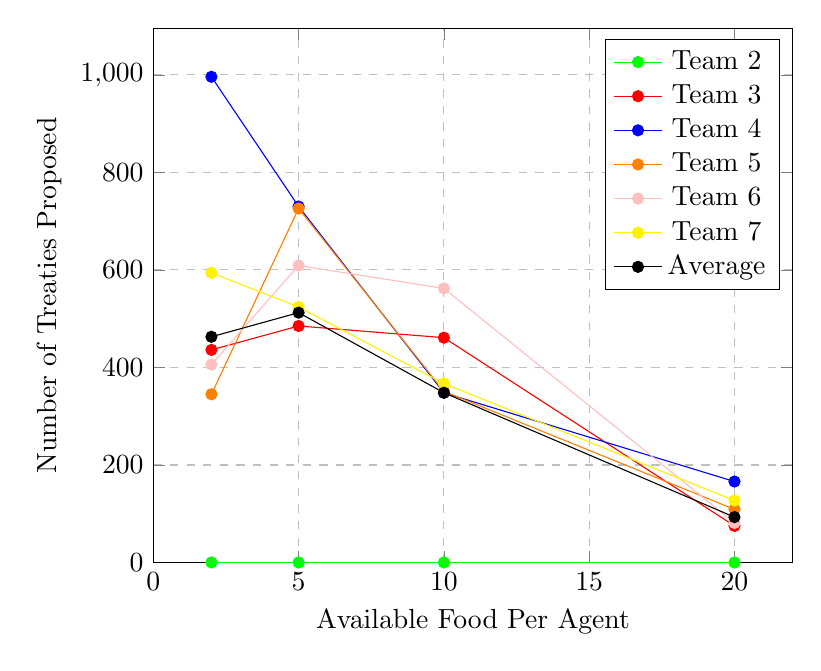
\begin{tikzpicture}
        \begin{axis}[
            width=0.8\textwidth,
            % axis y line*=left,
            ymin=0,
            xmin=0,
            xlabel=Available Food Per Agent,
            ylabel=Number of Treaties Proposed,
            ymajorgrids=true,
            xmajorgrids=true,
            grid style=dashed,
        ]
        \addplot[mark=*,green]
            coordinates{
                (2, 0)
                (5, 0)
                (10, 0)
                (20, 0)
            }; \label{leg:team2-scarcity}
        \addplot[mark=*,red]
            coordinates{
                (2, 436)
                (5, 485)
                (10, 461)
                (20, 75)
            }; \label{leg:team3-scarcity}
        \addplot[mark=*,blue]
            coordinates{
                (2, 996)
                (5, 730)
                (10, 348)
                (20, 166)
            }; \label{leg:team4-scarcity}
        \addplot[mark=*,orange]
            coordinates{
                (2, 345)
                (5, 726)
                (10, 351)
                (20, 109)
            }; \label{leg:team5-scarcity}
        \addplot[mark=*,pink]
            coordinates{
                (2, 406)
                (5, 609)
                (10, 562)
                (20, 81)
            }; \label{leg:team6-scarcity}
        \addplot[mark=*,yellow]
            coordinates{
                (2, 594)
                (5, 524)
                (10, 367)
                (20, 127)
            }; \label{leg:team7-scarcity}
        \addplot[mark=*,black]
            coordinates{
                (2, 462.83)
                (5, 512.33)
                (10, 348.17)
                (20, 93)
            }; \label{leg:average-scarcity}
        \addlegendimage{/pgfplots/refstyle=leg:team2-scarcity}\addlegendentry{Team 2}
        \addlegendimage{/pgfplots/refstyle=leg:team3-scarcity}\addlegendentry{Team 3}
        \addlegendimage{/pgfplots/refstyle=leg:team4-scarcity}\addlegendentry{Team 4}
        \addlegendimage{/pgfplots/refstyle=leg:team5-scarcity}\addlegendentry{Team 5}
        \addlegendimage{/pgfplots/refstyle=leg:team6-scarcity}\addlegendentry{Team 6}
        \addlegendimage{/pgfplots/refstyle=leg:team7-scarcity}\addlegendentry{Team 7}
        \addlegendimage{/pgfplots/refstyle=leg:average-scarcity}\addlegendentry{Average}
        \end{axis}
        \end{tikzpicture}
    \caption{Number of Treaties Proposed as Food Scarcity Decreases}
    \label{fig:team1-robustness-food-scarcity}
\end{figure}

\Cref{fig:team1-robustness-food-scarcity} illustrates the change in the frequency of treaty proposal as the constraints from the economy of scarcity are levied. The experiment enforces that there is 100 food initially available on the platform, with the number of agents parameterised to allow for an average amount of food per agent. This simulation lasts 400 turns.

The general tendency for this system is that, as the availability of food rises (and hence the economy of scarcity becomes less constrictive), the rate of treaty proposal decreases. We propose that this experiment yields insight into the importance of treaties, demonstrating that agents in general rely heavily on treaty formation to self organise when survivability is hindered by a lack of resources. Contrarily, as the food availability reaches an abundance, we see the rate of treaty proposal tend to 0, suggesting that agents are able to survive without the need for treaties as they offer little utility.

We also assert that this graph details the implied benefit of signing treaties: agents seem to value treaties as a means to fairer food distribution, wherein signing facilitates them receiving a greater proportion of food than they would otherwise receive without a treaty.

\begin{figure}[H] %Deaths As Food Scarcity Decreases with different agent combos added
    \centering
    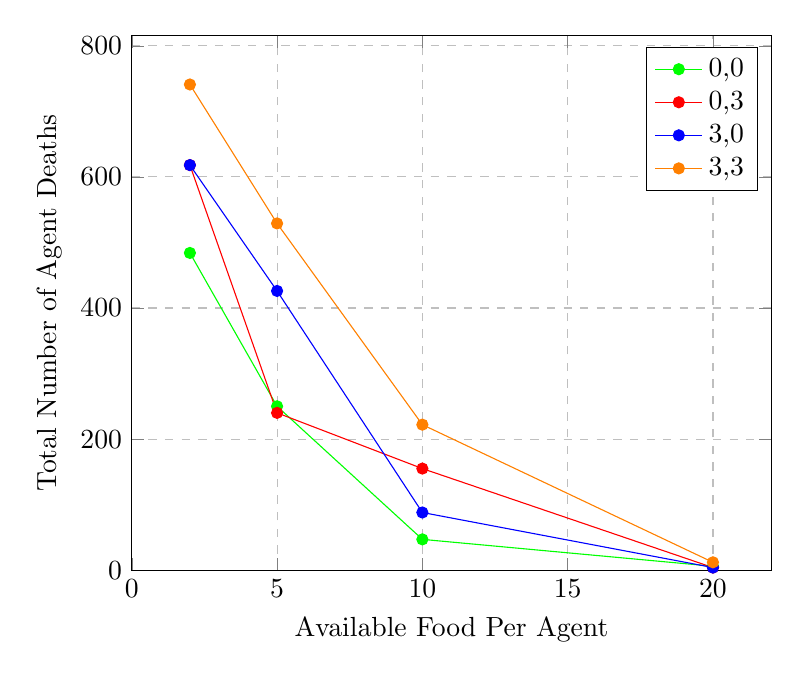
\begin{tikzpicture}
        \begin{axis}[
            width=0.8\textwidth,
            % axis y line*=left,
            ymin=0,
            xmin=0,
            xlabel=Available Food Per Agent,
            ylabel=Total Number of Agent Deaths,
            ymajorgrids=true,
            xmajorgrids=true,
            grid style=dashed,
        ]
        \addplot[mark=*,green]
            coordinates{
                (2, 484)
                (5, 250)
                (10, 47)
                (20, 6)
            }; \label{leg:scarcity00}
        \addplot[mark=*,red]
            coordinates{
                (2, 618)
                (5, 240)
                (10, 155)
                (20, 4)
            }; \label{leg:scarcity03}
        \addplot[mark=*,blue]
            coordinates{
                (2, 618)
                (5, 426)
                (10, 88)
                (20, 4)
            }; \label{leg:scarcity30}
        \addplot[mark=*,orange]
            coordinates{
                (2, 741)
                (5, 529)
                (10, 222)
                (20, 12)
            }; \label{leg:scarcity33}
        \addlegendimage{/pgfplots/refstyle=leg:scarcity00}\addlegendentry{0,0}
        \addlegendimage{/pgfplots/refstyle=leg:scarcity03}\addlegendentry{0,3}
        \addlegendimage{/pgfplots/refstyle=leg:scarcity30}\addlegendentry{3,0}
        \addlegendimage{/pgfplots/refstyle=leg:scarcity33}\addlegendentry{3,3}
        \end{axis}
        \end{tikzpicture}
    \caption{The total number of deaths in systems with different combinations of selfish and random agents added as food per agent increases. The number of each disruptive agent added to each system is show in the legend in the form (number of selfish agents, number of random agents)}
    \label{fig:team1-robustness-food-scarcity-disruptive-agents}
\end{figure}

\Cref{fig:team1-robustness-food-scarcity-disruptive-agents} shows how the number of deaths is affected when different disruptive agents are added. It shows that, as expected, the number of deaths is higher when disruptive agents are present. However, the effect of selfish agents and random agents seem to be similar which suggests that it it not the amount of food being taken by the agents that is disruptive, rather it is the fact that they do not communicate that causes a higher death rate. This makes it harder to self organise and makes it much harder to survive in the tower. 
And by making it harder to survive in the tower, the chances of reaching a stable system are also decreased when disruptive agents are added, the only system to stabilise with 10 food per agent was the one with no disruptive agents, all systems were stable with a tower of 20 food per agent.
Interestingly
\subsection{Conclusion}
\label{subsec: E1-Conclusion}
This experiment shows the importance of treaties and communication for the survival of the agents in the tower.And so this shows that self organisation is a key factor in the ability of the tower to reach a stable state.

\section{Experiment 2}
\label{subsec: Experiment 2}
\subsection{Aims}
\label{subsec: E2-Aims}
The aim of this experiment is to vary the number of ticks per floor and reshuffle period and observe the effects of this on tower stability and ability to self organise.
\subsection{Results and Discussion}
\label{subsec: E2-Results and Discussion}

\begin{figure}[H] %Number of Deaths As Shuffle Period Decreases
    \centering
    \begin{minipage}{0.8\textwidth}
        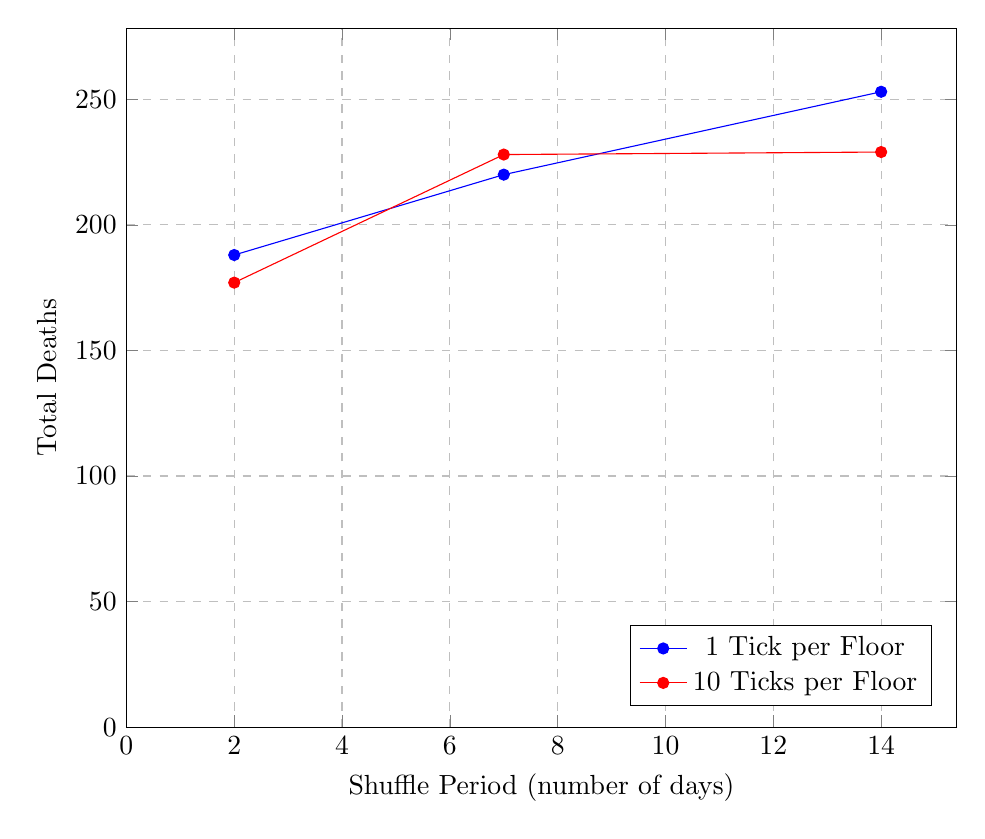
\begin{tikzpicture}
            \begin{axis}[
                width=\textwidth,
                % axis y line*=left,
                ymin=0,
                xmin=0,
                xlabel=Shuffle Period (number of days),
                ylabel=Total Deaths,
                ymajorgrids=true,
                xmajorgrids=true,
                grid style=dashed,
                legend pos=south east
            ]
            \addplot[mark=*,blue]
                coordinates{
                    (14, 253)
                    (7, 220)
                    (2, 188)
                }; \label{leg:reshuffle-ticks-per-floor1}
            \addplot[mark=*,red]
                coordinates{
                    (14, 229)
                    (7, 228)
                    (2, 177)
                }; \label{leg:reshuffle-ticks-per-floor10}
            \addlegendimage{/pgfplots/refstyle=leg:reshuffle-ticks-per-floor1}
            \addlegendentry{1 Tick per Floor}
            \addlegendimage{/pgfplots/refstyle=leg:reshuffle-ticks-per-floor10}\addlegendentry{10 Ticks per Floor}
            \end{axis}
        \end{tikzpicture}
    \end{minipage}
    \caption{Total Deaths in the Tower as Reshuffle Period Increases}
    \label{fig:Number-of-Deaths-As-Shuffle-Period-Decreases}
\end{figure}


For this reason, we propose that it is the rapid redistribution of agents throughout the tower, allowing them to experience varying levels of available food that accounts for the disparity in survival rate: if an agent is consistently assigned to a low floor, they have a low chance of being satisficed if all agents act individually. Having a rapid reshuffle period results in a higher probability of reaching a higher floor, allowing for the agent to replenish its health. 

The average age of agents, denoted by \Cref{fig:Average-Age-as-Shuffle-Period-Decreases}, can be see to follow the inverse trend to death rates which is as expected. This trend being, that the longer the reshuffle period the lower the average age of an agent at death. 
\begin{figure}[H] %Average Age As Shuffle Period Decreases
    \centering
    \begin{minipage}{0.8\textwidth}
        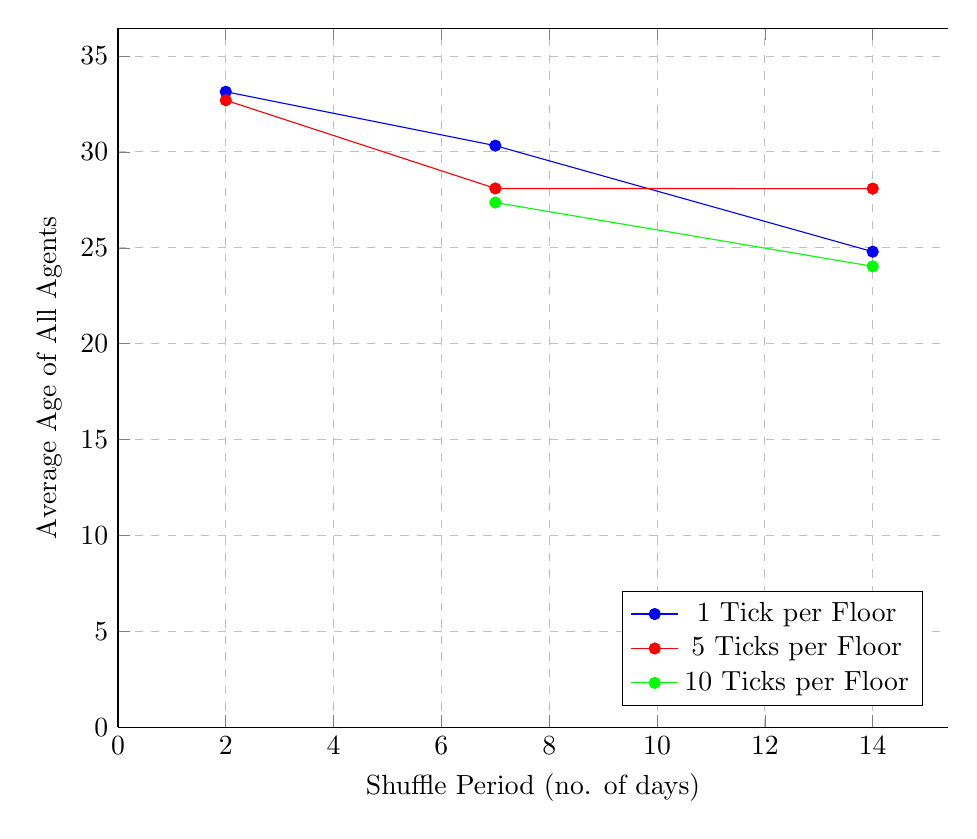
\begin{tikzpicture}
            \begin{axis}[
                width=\textwidth,
                axis y line*=left,
                ymin=0,
                xmin=0,
                xlabel=Shuffle Period (no. of days),
                ylabel=Average Age of All Agents,
                ymajorgrids=true,
                xmajorgrids=true,
                grid style=dashed,
                legend pos=south east
            ]
            \addplot[mark=*,blue]
                coordinates{
                    (14, 24.798)
                    (7, 30.327)
                    (2, 33.138)
                }; \label{leg:reshuffle-ticks-per-floor1}
            \addplot[mark=*,red]
                coordinates{
                    (14, 28.087)
                    (7, 28.096)
                    (2, 32.695)
                }; \label{leg:reshuffle-ticks-per-floor10}
            \addplot[mark=*,green]
                coordinates{
                    (14, 24.034)
                    (7, 27.36)
                }; \label{leg:reshuffle-ticks-per-floor5}
            \addlegendimage{/pgfplots/refstyle=leg:reshuffle-ticks-per-floor1}
            \addlegendentry{1 Tick per Floor}
            \addlegendimage{/pgfplots/refstyle=leg:reshuffle-ticks-per-floor5}
            \addlegendentry{5 Ticks per Floor}
            \addlegendimage{/pgfplots/refstyle=leg:reshuffle-ticks-per-floor10}\addlegendentry{10 Ticks per Floor}
            \end{axis}
        \end{tikzpicture}
    \end{minipage}
    \caption{Average Age in the Tower as Reshuffle Period Increases}
    \label{fig:Average-Age-as-Shuffle-Period-Decreases}
\end{figure}

\Cref{fig:Total-Accepted-Treaties-As-Shuffle-Period-Decreases} and \Cref{fig:Total-Rejected-Treaties-As-Shuffle-Period-Decreases} show that significant numbers of treaties are being exchanged at all reshuffle periods, demonstrating that a social network is being formed. However, as the reshuffle period decreases the number of treaties accepted and rejected and so the total number of treaties proposed decreases. This is as expected since, if agents have the same neighbours for longer periods of time, they need to exchange fewer new treaties, given that each proposed treaty will be agreed upon by neighbours for longer and so neighbours will not need to send each other new treaties. 

\begin{figure}[H] %Total Accepted Treaties As Shuffle Period Decreases
    \centering
    \begin{minipage}{0.8\textwidth}
        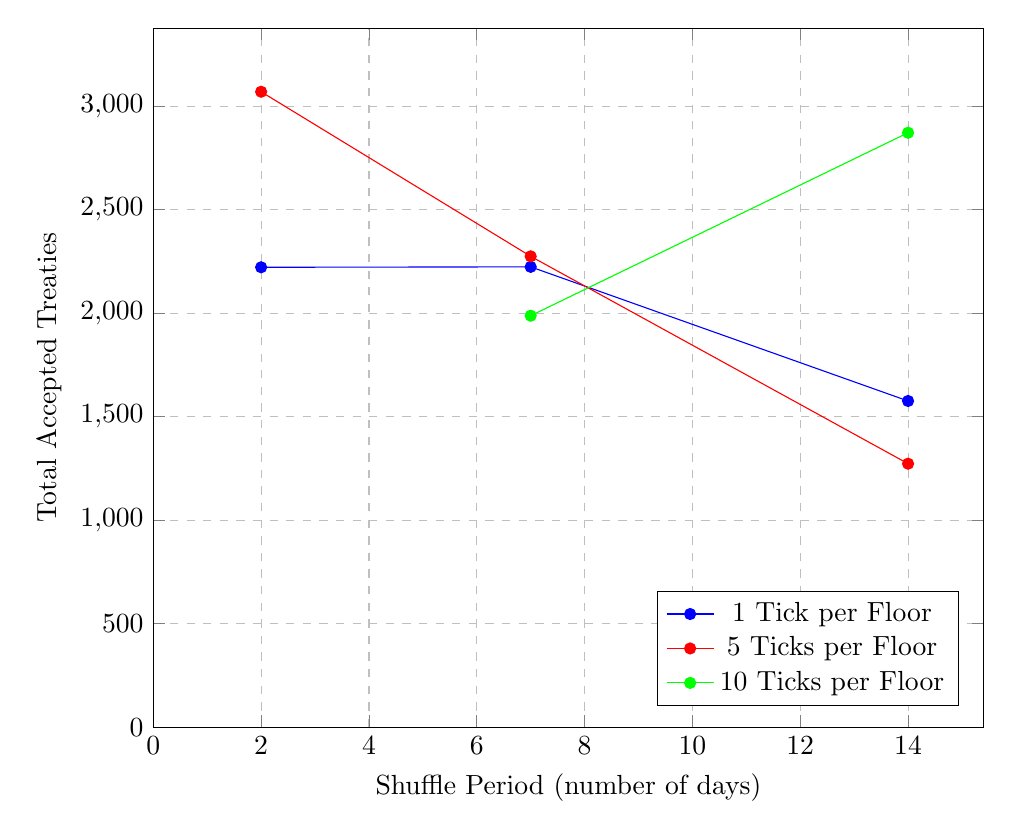
\begin{tikzpicture}
            \begin{axis}[
                width=\textwidth,
                % axis y line*=left,
                ymin=0,
                xmin=0,
                xlabel=Shuffle Period (number of days),
                ylabel=Total Accepted Treaties,
                ymajorgrids=true,
                xmajorgrids=true,
                grid style=dashed,
                legend pos=south east
            ]
            \addplot[mark=*,blue]
                coordinates{
                    (14, 1576)
                    (7, 2224)
                    (2, 2222)
                }; \label{leg:reshuffle-ticks-per-floor1}
            \addplot[mark=*,red]
                coordinates{
                    (14, 1273)
                    (7, 2275)
                    (2, 3070)
                }; \label{leg:reshuffle-ticks-per-floor10}
            \addplot[mark=*,green]
                coordinates{
                    (14, 2872)
                    (7, 1988)
                }; \label{leg:reshuffle-ticks-per-floor5}
            \addlegendimage{/pgfplots/refstyle=leg:reshuffle-ticks-per-floor1}
            \addlegendentry{1 Tick per Floor}
            \addlegendimage{/pgfplots/refstyle=leg:reshuffle-ticks-per-floor5}
            \addlegendentry{5 Ticks per Floor}
            \addlegendimage{/pgfplots/refstyle=leg:reshuffle-ticks-per-floor10}\addlegendentry{10 Ticks per Floor}
            \end{axis}
        \end{tikzpicture}
    \end{minipage}
    \caption{Total Accepted Treaties As Shuffle Period Decreases}
    \label{fig:Total-Accepted-Treaties-As-Shuffle-Period-Decreases}
\end{figure}

\begin{figure}[H] %Total Rejected Treaties As Shuffle Period Decreases
    \centering
    \begin{minipage}{0.8\textwidth}
        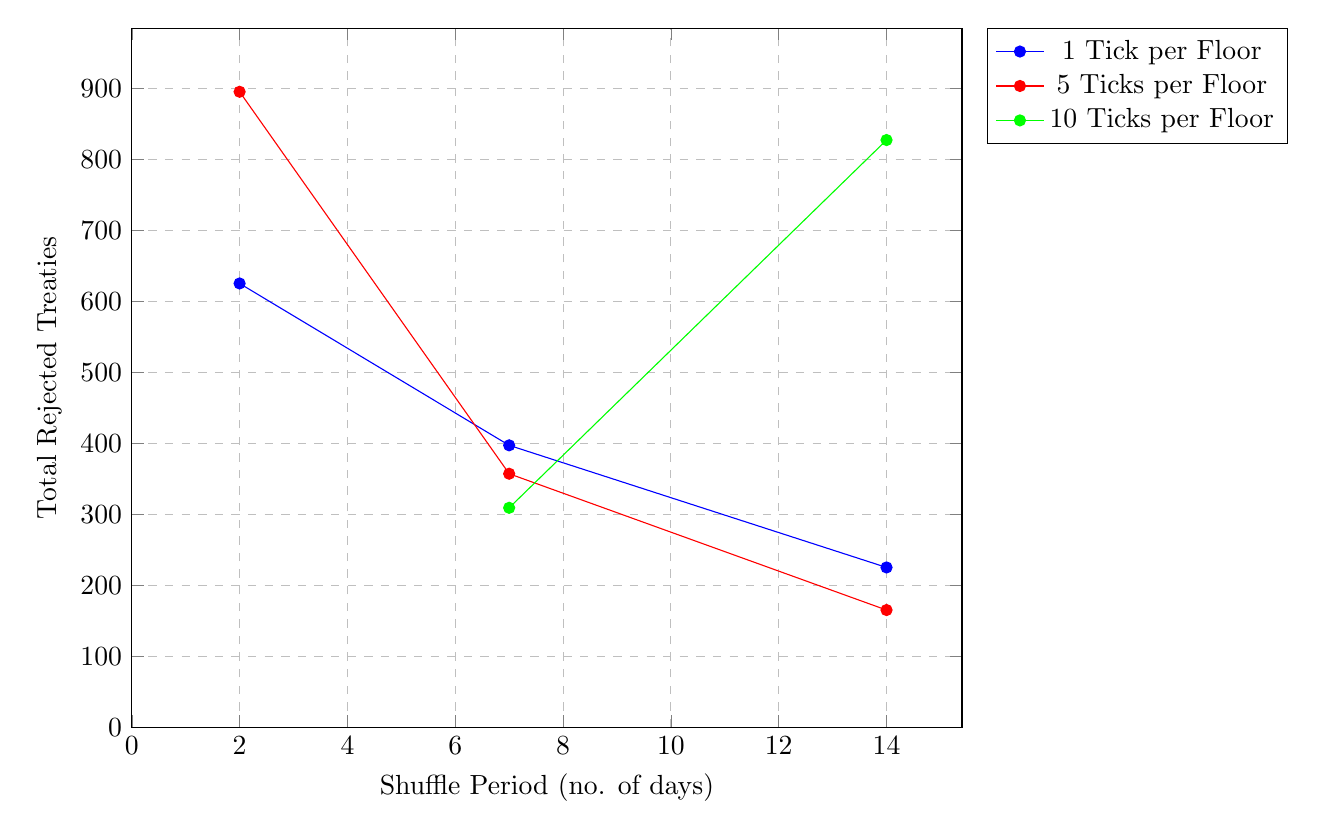
\begin{tikzpicture}
            \begin{axis}[
                width=\textwidth,
                % axis y line*=left,
                ymin=0,
                xmin=0,
                xlabel=Shuffle Period (no. of days),
                ylabel=Total Rejected Treaties,
                ymajorgrids=true,
                xmajorgrids=true,
                grid style=dashed,
                legend pos=outer north east
            ]
            \addplot[mark=*,blue]
                coordinates{
                    (14, 225)
                    (7, 397)
                    (2, 625)
                }; \label{leg:reshuffle-ticks-per-floor1}
            \addplot[mark=*,red]
                coordinates{
                    (14, 165)
                    (7, 357)
                    (2, 895)
                }; \label{leg:reshuffle-ticks-per-floor10}
            \addplot[mark=*,green]
                coordinates{
                    (14, 827)
                    (7, 309)
                }; \label{leg:reshuffle-ticks-per-floor5}
            \addlegendimage{/pgfplots/refstyle=leg:reshuffle-ticks-per-floor1}
            \addlegendentry{1 Tick per Floor}
            \addlegendimage{/pgfplots/refstyle=leg:reshuffle-ticks-per-floor5}
            \addlegendentry{5 Ticks per Floor}
            \addlegendimage{/pgfplots/refstyle=leg:reshuffle-ticks-per-floor10}\addlegendentry{10 Ticks per Floor}
            \end{axis}
        \end{tikzpicture}
    \end{minipage}
    \caption{Total Rejected Treaties As Shuffle Period Decreases}
    \label{fig:Total-Rejected-Treaties-As-Shuffle-Period-Decreases}
\end{figure}

\subsection{Conclusion}
\label{subsec: E2-Conclusion}
The change in reshuffle period and number of ticks per floor does not have a significant impact on the ability of the agents to self organise. However, increasing the reshuffle period does increase the overall deaths and so would make reaching stability more difficult.



\input{011_results/011_results}
\input{012_discussion/012_discussion}
\chapter{Conclusion}\label{conclusion}

This project has involved the design and implementation of six different agents with various strategies to self-organise and solve a common resource management problem, where the common resource, in this case, is the scarcity of food available to agents in the tower.

It has been shown that in order for self-organisation to be achieved within the tower, communication is necessary between all present agents through both messaging and the signing of treaties. Agents which were succesful in achieving self-organisation did so by gaining knowledge of both the tower and other agents, and applying this knowledge appropriately. Without this, the most logical behaviour of an agent is to act purely selfishly, giving itself the best chance of survival in a random system.
\input{014_future_work/014_future_work}
% Appendix
\appendix
\chapter{Appendix}\label{supplementary_material}

Appendix Section. Org chart could go here. Potentialy could include implementation details.

% References
\newpage
\nocite{*}
\bibliography{references} 
\bibliographystyle{IEEEtranN}

%%%%%%%%%%%%%%%%%%%%%%%%%%%%%%%%%%%%%%%%%%%%%%%%%%%%%%%%%%%%%%%%%
%                        Document End                           %
%%%%%%%%%%%%%%%%%%%%%%%%%%%%%%%%%%%%%%%%%%%%%%%%%%%%%%%%%%%%%%%%%
\end{document}
